\documentclass[10pt,a4paper]{article}
\usepackage{float}	
\usepackage{graphicx}
\usepackage{url}
\usepackage{fullpage}
\usepackage{microtype}
\usepackage[toc,page]{appendix}
\usepackage[utf8]{inputenc}
\usepackage[parfill]{parskip}
\usepackage[para,online]{threeparttable}
\usepackage{booktabs}
\usepackage{hyperref}
\usepackage{listings}
\usepackage[justification=centering]{caption}
\usepackage{textcomp,gensymb}
\usepackage{amsmath}
\usepackage[gen]{eurosym}
\usepackage{color,soul}
\usepackage{pdfpages}
\usepackage{chngcntr}
\usepackage{graphicx}
\usepackage{subfig}
\usepackage{fancyhdr}
\usepackage{tikz}

\title{Latex Template}

\begin{document}
\numberwithin{equation}{section}
\numberwithin{figure}{section}
\numberwithin{table}{section}
\setlength{\headheight}{15.2pt}
\pagestyle{fancy}
\fancyhf{}
\renewcommand{\headrulewidth}{0pt}
\renewcommand{\footrulewidth}{0.4pt}
\fancyfoot[L]{TU/e}
\fancyfoot[R]{Page \thepage}

\lstdefinelanguage{chi}
  {morekeywords={if,then,select,alt,dist,proc,type,tuple,int,real,const,while,delay,end,chan,true,model,run,for,write,writeln,pass,unwind,in,list,time},
   morestring=[d]"
  }

%%Check whole page!

\begin{titlepage}
	\centering
	\vspace*{2cm}
	{\scshape\Large Eindhoven University of Technology \par}
	\vspace{.5cm}
	{\scshape\large Department of Mechanical Engineering\\ Energy Technology\par}
	\vspace{2.5cm}
	{\LARGE\bfseries Bachelor Eind Project \par}
    \vspace{0.3cm}
    {\scshape \large Optimizing Energy Performance}\\
	\vspace{.25cm}
	{\large\itshape Eindhoven, 2017 \par}
	\vfill
	
\begin{flushleft}
	\begin{tabular}{ll}
	\\		B.L. Klein Holkenborg & 0892107
 	\end{tabular}
    \vspace{1.5cm}
\end{flushleft} 
		
\end{titlepage}
\section*{List of symbols}
\thispagestyle{empty}
\begin{tabular}{| p{4cm} | p{4cm} | p{4cm} | p{4cm} |}
\hline
\large\textbf{Symbol} & \large\textbf{Variable} & \large\textbf{Unit} & \large\textbf{Unit abbreviation} \\
\hline\hline
\textit{A}			& Surface			& meter squared			    & m$^{2}$ \\ \hline
\textit{d}			& Diameter			& meter							& m   \\ \hline
\textit{E} 			& Young's modulus 	& Pascal 						& Pa  \\ \hline
\textit{h}			& Mesh size			& one per millimeter			& 1/mm\\ \hline
\textit{L}			& Length			& meter							& m	  \\ \hline
\textit{r} 			& Radius 			& meter 						& m   \\ \hline
\textit{R$_{i}$}	& Inner radius		& meter							& m   \\ \hline
\textit{R$_{o}$}	& Outer radius		& meter							& m   \\ \hline
\textit{t}			& Time				& seconds						& sec \\ \hline
\textit{T}			& Temperature		& degree Celsius	   &\textdegree C \\ \hline
\textit{T} 			& Temperature 		& Kelvin 						& K   \\ \hline
\textit{T$_{ambient}$} & Ambient temperature & degree Celsius  &\textdegree C \\ \hline
\textit{T$_{i}$}	& Inner temperature	& degree Celsius	   &\textdegree C \\ \hline
\textit{T$_{o}$}	& Outer temperature	& degree Celsius	   &\textdegree C \\ \hline
\textit{$\alpha$} 	& Thermal expansion coefficient & one per Kelvin 	& 1/K \\ \hline
\textit{$\epsilon$} & Deformation		& meter					& m  \\ \hline
\textit{$\sigma$} 	& Stress 			& Pascal 						& Pa  \\ \hline
\textit{$\sigma_{rr}$} & Radial stress 	& Pascal 						& Pa  \\ \hline
\textit{$\sigma_{\theta \theta}$} & Tangential stress & Pascal 			& Pa  \\ \hline


\end{tabular}

\newpage
\tableofcontents
\thispagestyle{empty}
\newpage
\section*{Introduction}
\addcontentsline{toc}{section}{Introduction}
\label{introduction}

\newpage
\section{Lithium-Ion Batteries}
\label{Chap:lithium_ion_batteries}
Before a battery is chosen and investigated in detail, it is important to know exactly how such a battery works. Key parameters have to be explained and the many different options of batteries have to be discussed. In this section, a general explanation of lithium-ion batteries will be given as well as an explanation of some common commercial configurations in which they come.

\subsection{What is a lithium-ion battery}
Lithium-ion batteries work like most other batteries available. Batteries now-a-days consist out of a cathode, anode, electrolyte, separator and current collectors. A schematic drawing of a battery layer is given in figure \ref{Fig:Li-Ion_Schematic}.

\begin{figure} [H]
 	\centering	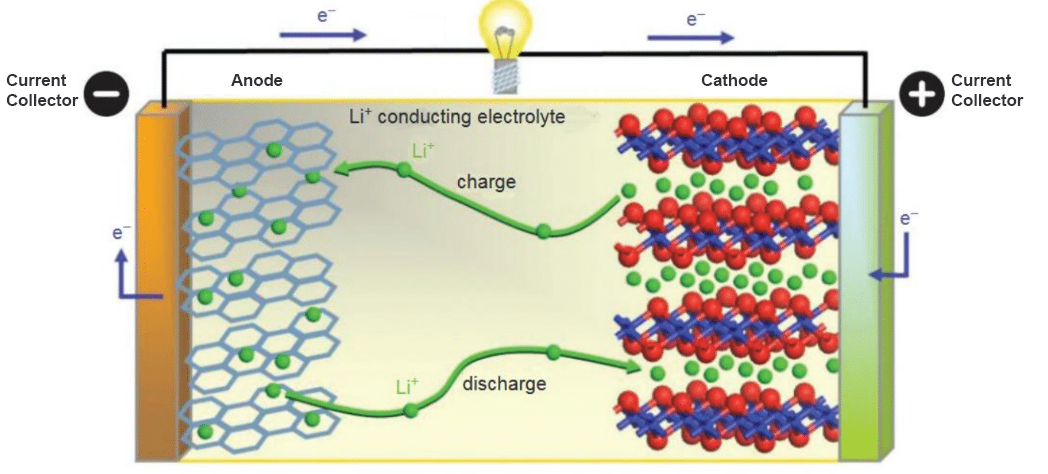
\includegraphics[width=0.8\linewidth]{Figures/scematic.PNG}
 	\caption{Schematic drawing of the lithium-ion battery layer}
    \label{Fig:Li-Ion_Schematic}
\end{figure}

When discharging, lithium-ion particles (hence lithium-ion batteries) flow from the anode to the cathode material. The anode and cathode material is structured so that the lithium-ion particles can be released and taken into the layered structure. A process called intercalation. Some common materials that inherit this structure are carbon compounds like graphite for the anode, and metallic oxides like LiCoO$_2$ for the cathode. When the charged lithium particles transfer from anode to cathode, an potential difference is created causing electrons to flow as well.

However, electrons need to flow through an external circuit, as to allow some device to be powered. Thus a non-conductive barrier must be created that allows lithium-ions to be transferred, but stops electrons from going through. An aqueous medium called the electrolyte allows the transfer of lithium particles. This medium is a lithium salt like LiPF$_6$ which is solved into a EC:DEC:DMC solvent usually. The specific materials and ratios used may vary however. A porous polymer membrane gelled with this electrolyte is then placed in the middle of the electrodes. This allows lithium-ions to travel through, but stops electrons from doing so.

The electrodes are coated onto metal current collectors. Current collectors form the positive and negative terminal of a battery. Because of the potential difference in the electrodes, electrons then flow through the current collector through the external circuit and back into the battery again, equaling the potential difference (causing a voltage drop explained in \textbf{REFERENEN NAAR VOLTAGE DROP}).

Typically, a battery's electrodes are defined during discharge. When someone refers to the cathode material, this means the person refers to the material that is the cathode during discharge. However during charge, the electrodes switch. The discharging anode becomes the charging cathode, and the other way around for the discharging cathode. During charge, lithium ions flow back to their original side. This is the mechanism that allows lithium batteries to be recharged. A problem however is that lithium batteries have only a limited amount of recharges after which they become unstable and a lacking performance. This is due to mechanism described later in section \ref{Chap:Battery_Safety}.

\subsection{Chemistries}
There are many different lithium battery commercially available. They mostly differ in mechanical structure and in their chemistry. Both may have a significant impact on battery performance. First, a select few popular commercial chemistries will be looked into, after which different mechanical structures will be detailed. 

Although all components of a lithium battery can be changed in material, manufacturers and data-sheets will almost always refer to the cathode material as to define the battery its chemistry. Why that is, is that all other components do not have good commercially available alternatives. Almost all anodes are made out of graphite. Today incorporating silicone additives into the graphene is ongoing, yet still commercially unavailable. Graphene also is being looked into, however still mainly graphite is used. \\
Cathode material however consists out of metal oxides, of which there are many different options. Each of these have different impact on the performance of a battery. Since mainly the cathode material impacts the batteries performance electrochemically, the cathode material is thus referred to as to define the batteries chemistry \cite{cathode}. The cathode impacts energy density, power density, safety and lifespan. Also choice of cathode impacts the costs, depending on the cathode material, it can make up 25$\%$ of the total battery production costs. \cite{cathode}\cite{cobalt}

\begin{figure} [H]
 	\centering
 	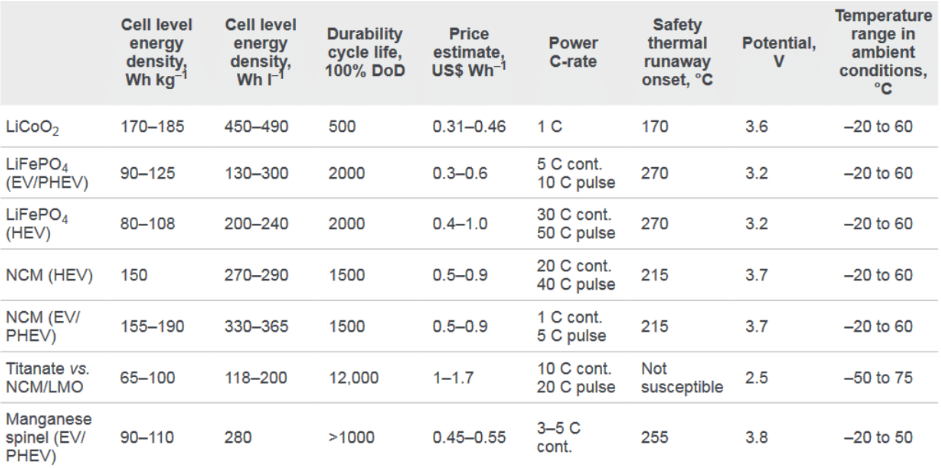
\includegraphics[width=0.9\linewidth]{Figures/chemistry_table.PNG}
 	\caption{Battery cell properties with different chemistries (from \cite{slides})}
    \label{Fig:Chemistry_table}
\end{figure}

In figure \ref{Fig:Chemistry_table}, a table is given that indicates different properties of battery cells with different cathode chemistries. Below, a few common chemistries will be explained.\\
\begin{enumerate}
\item LCO - LiCoO$_2$\\
The Lithium Cobalt Oxide (LCO) chemistry is the most common type of lithium-ion battery. It owes its popularity by the high energy density both by weight and volume. In fact, by volume it inherits one of the highest energy densities. This is really useful for many applications as design space is often limited. For the industry it is currently the cheapest chemistry as well. Note however that this is mainly due to mass fabrication since cobalt actually is relatively expensive since cobalt has no primary source. It is obtained as a byproduct of copper and nickel mining \cite{cobalt}.\\
LCO's advantages however come with disadvantages. With each cycle, LCO batteries have a fast decline in performance and is most vulnerable to thermal runaway compared to other chemistries. Thermal runaway is when a battery cell decomposes in a violent manner caused by a chain of exothermic reactions.

\item LMO - LiMn$_2$O$_4$
\textit{Kort uitleggen}

\item NMC - LiNiMnCoO$_2$
\textit{Kort uitleggen}

\item NCA - LiNiCoAlO$_2$
\textit{Kort uitleggen}

\end{enumerate}

\subsection{Battery Types}
Batteries come in many different mechanical designs, which each come with specific characteristics. Some common configurations used in Radio controlled Vehicles (RVs) will be explained.
\begin{enumerate}
\item Cylindrical\\
The cylindrical cell is a widely used battery type. Cylindrical cells are easy and cheap to produce, enable different safety options to be implemented, are mechanically strong and offer decent thermal cooling. A cylindrical cell is a wound up battery layer enclosed in a metal enclosure. On both ends of the cell the terminals are situated, in order to connect to an external circuit. The battery is schematically drawn in figure \ref{Fig:Cylindrical_Cell}. 
\begin{figure} [H]
 	\centering	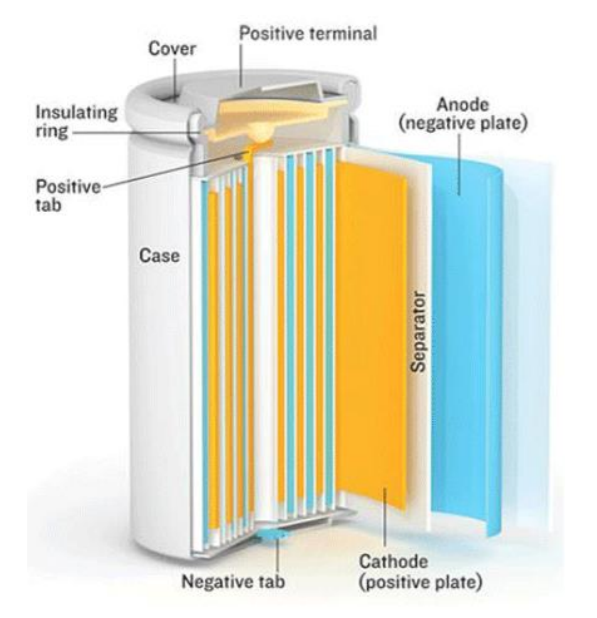
\includegraphics[width=0.5\linewidth]{Figures/cylindrical.PNG}
 	\caption{Schematic drawing of a cylindrical battery cell}
    \label{Fig:Cylindrical_Cell}
\end{figure}
It is said above, several safety options can be implemented in a cylindrical cell. The option to build internal safety mechanisms is quite an advantage over other types of cells since this can be fabricated during the battery creation. Most other cells can only have external safety devices to be attached to the external circuit, which requires assembly by users. Safety measures are explained in more detail in section \ref{Chap:Battery_Safety}. \\
Some disadvantages of cylindrical cells are that their size is limited, and thus their capacity. For large demanding applications, many of such batteries have to be combined. The assembly of such a battery pack may prove difficult and prone to errors. The optimal packing efficiency in a battery pack also is suboptimal. The packing efficiency can be approximated by the optimal packing of circles in a 2-dimensional field which is proven to be a hexagonal pattern \cite{optimal_packing} as seen in figure \ref{Fig:optimal_packing}.
\begin{figure} [H]
 	\centering	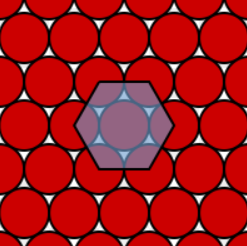
\includegraphics[width=0.5\linewidth]{Figures/optimal_packing.PNG}
 	\caption{Optimal packing of circles in a 2-dimensional space}
    \label{Fig:optimal_packing}
\end{figure}
The optimal packing is then calculated by formula \ref{Eq:optimal_packing}.
\begin{equation}
\frac{\pi}{\sqrt{12}} = 0.9069
\label{Eq:optimal_packing}
\end{equation}
Cylindrical cell packing ensures available cooling surface, though also a decrease of energy density in a battery pack. However, this energy density is further decreased since space is also lost by the metal enclosure and the empty center in a cylindrical cell. Additionally, the weight in a cylindrical cell battery pack is relatively high because of all the metal enclosures.\\
Even though cylindrical cells may thus seem undesirable for large battery packs, their cost, reliability and thermal management combined make for a combination that electric vehicle manufacturers choose for, like the Tesla company does for its vehicles \cite{battery_choice}.
\item Prismatic\\
The prismatic cell is basically a cylindrical cell but wound flattened. This makes for a more square shape which enables for a square metal housing. The square housing makes for a better packing density. They are however harder and more expensive to make than cylindrical cells and furthermore do not provide the same ability of incorporating certain safety mechanisms because of their square and asymmetric shape. Since the rise of pouch cells, Prismatic cells are becoming less popular now that the benefit of having a square shape is not unique to the prismatic cell anymore.
\item Pouch (LiPo)\\
Pouch cells have a distinctly different construction than cylindrical en prismatic cells have. Cylindrical and prismatic cells have a single sheet of battery layer that is wound up. Pouch cells on the other hand have a laminar layer. Battery layers are stacked upon each other and then sealed in an aluminum foil, with two metal connection terminal tabs sticking out. A schematic drawing is given in figure \ref{Fig:lipo_cell}, as well as an illustration of pouch cells.
\begin{figure}[H]
  \centering
  \subfloat[Pouch cell schematic.]{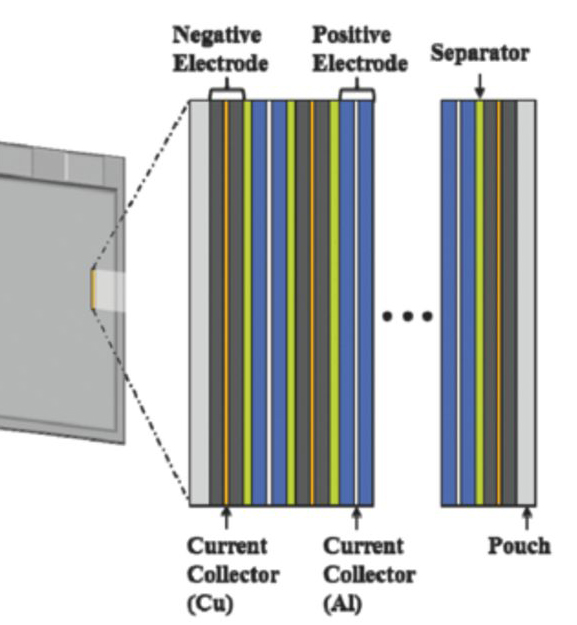
\includegraphics[width=0.5\textwidth]{Figures/Lipo_schematic.jpg}\label{Fig:lipo_schematic}}
  \hfill
  \subfloat[Pouch cells illustrated.]{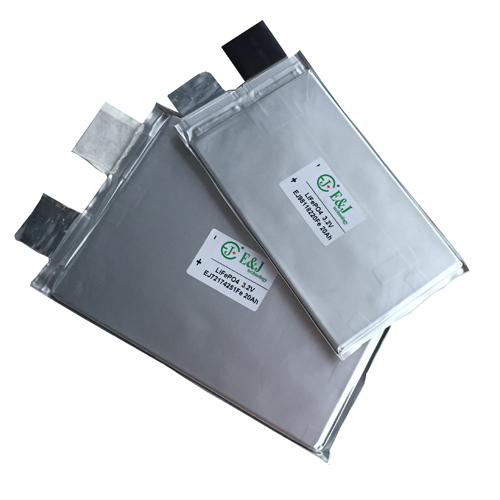
\includegraphics[width=0.5\textwidth]{Figures/Lipo_Cells.jpg}\label{Fig:lipo_cells}}
  \caption{Pouch cells}
  \label{Fig:lipo_cell}
\end{figure}
Because of their laminar origin, they can be created in many different shapes and sizes. Commercially they are almost always sold in rectangular shapes since this is cheap to produce and often a fit shape for their application. Their size is also variable from just as few as 10 mAh, up to more than 50Ah. This is because the layer sheets can be made as big as needed, and can also be stacked as many times as wished. This might cause thermal problems however, but it is possible if needed.\\
Pouch cells are optimized for power and energy density. Besides the active material, only current collectors and a thin aluminum foil is adding weight to the battery. This makes for a very weight and volume efficient design. A problem however is that a pouch cell has no hard metal casing, and thus is vulnerable to penetration. Also, lithium batteries swell as they age because of decomposition of active material. In hard metal casing this is suppressed, but in aluminum foil cased cells, batteries will expand. \\
Pouch cells have a very wide functionality. They are used in credit cards to provide power to its chip, but also function in electronic vehicles like the Nissan Leaf. \\
Commonly pouch cells are referred to as Lithium Polymer cells because of the laminar structure and their polymer separators. True Lithium Polymer cells however are cells with a polymer electrolyte. These however are not commercially available because of conductivity problems. The term LiPo for commercial cells as of now is thus incorrect \cite{Sequeira20103} \cite{lithium_batteries2}.
\item Solid-State\\
\textit{eerst meer informatie over zoeken, geen hoge prioriteit}
\end{enumerate}


%\begin{figure} [H]
% 	\centering
% 	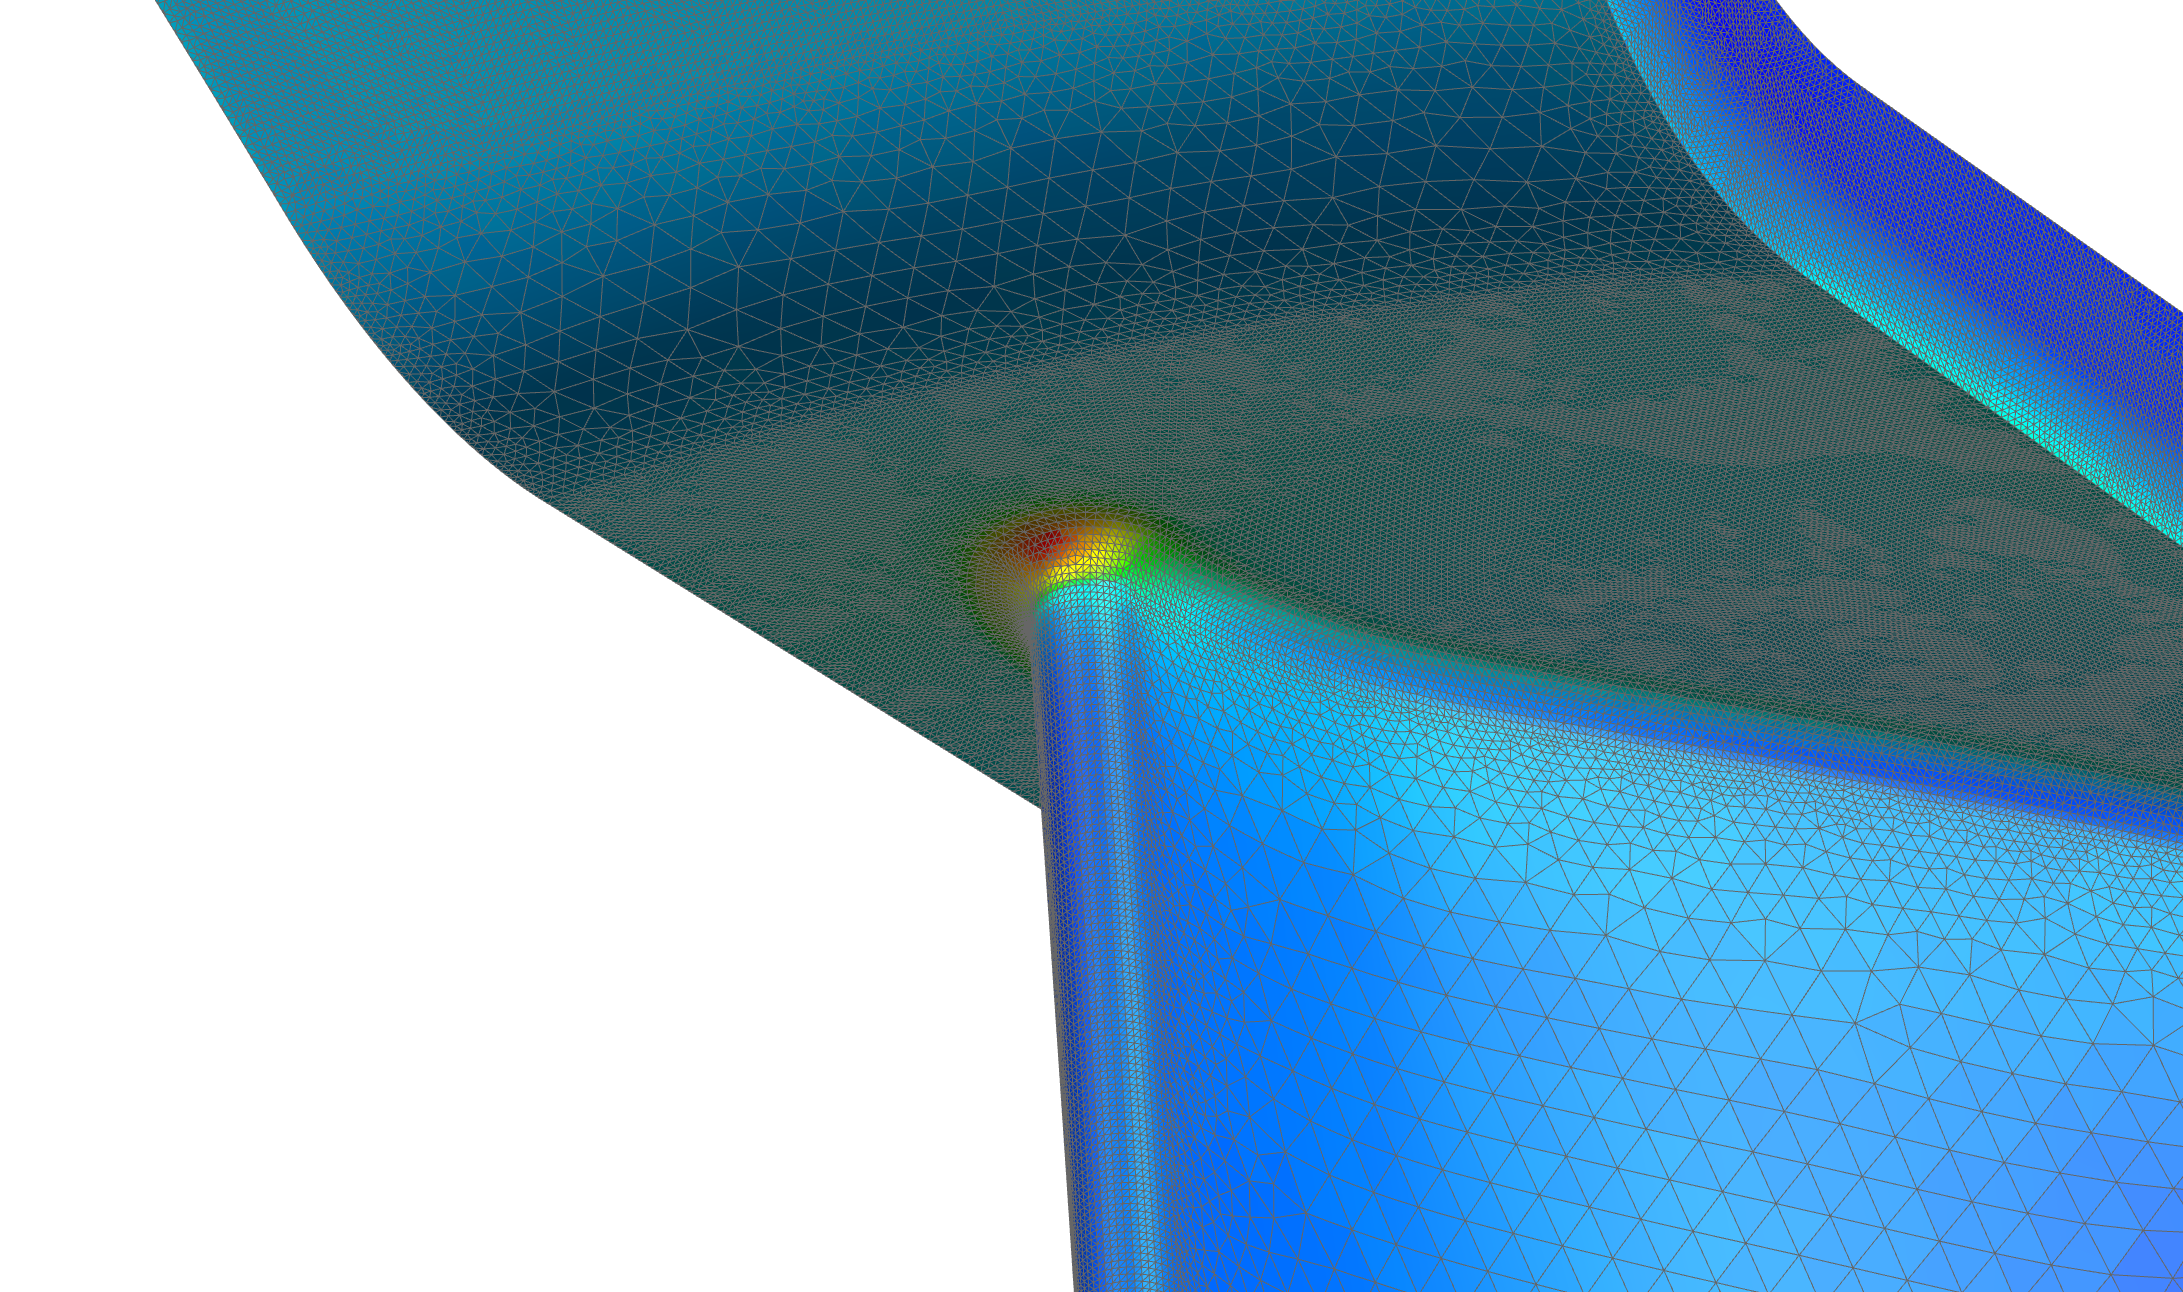
\includegraphics[width=0.8\linewidth]{Figures/stator_shutdown.png}
% 	\caption{Maximum stress during shut-down condition}
%    \label{stator1}
% \end{figure}

placeholder
\newpage
\section{Battery Safety}
\label{Chap:Battery_Safety}
Hier safety eigenschappen bepalen, zodat men hier naar kan kijken als reference sheet.
\subsection{Mechanical stability}


\subsection{Thermal stability}
\label{Sub:Thermal_Stability}
High temp effects
Low temp effects
Stacked effect
Tabs


\subsection{Electrical stability}
\label{Sub:Electrical_Stability}
Too high volt
Too low volt
High discharge
High charge
Aging
Storage
Cell balancing
Control boards

%\begin{figure} [H]
% 	\centering
% 	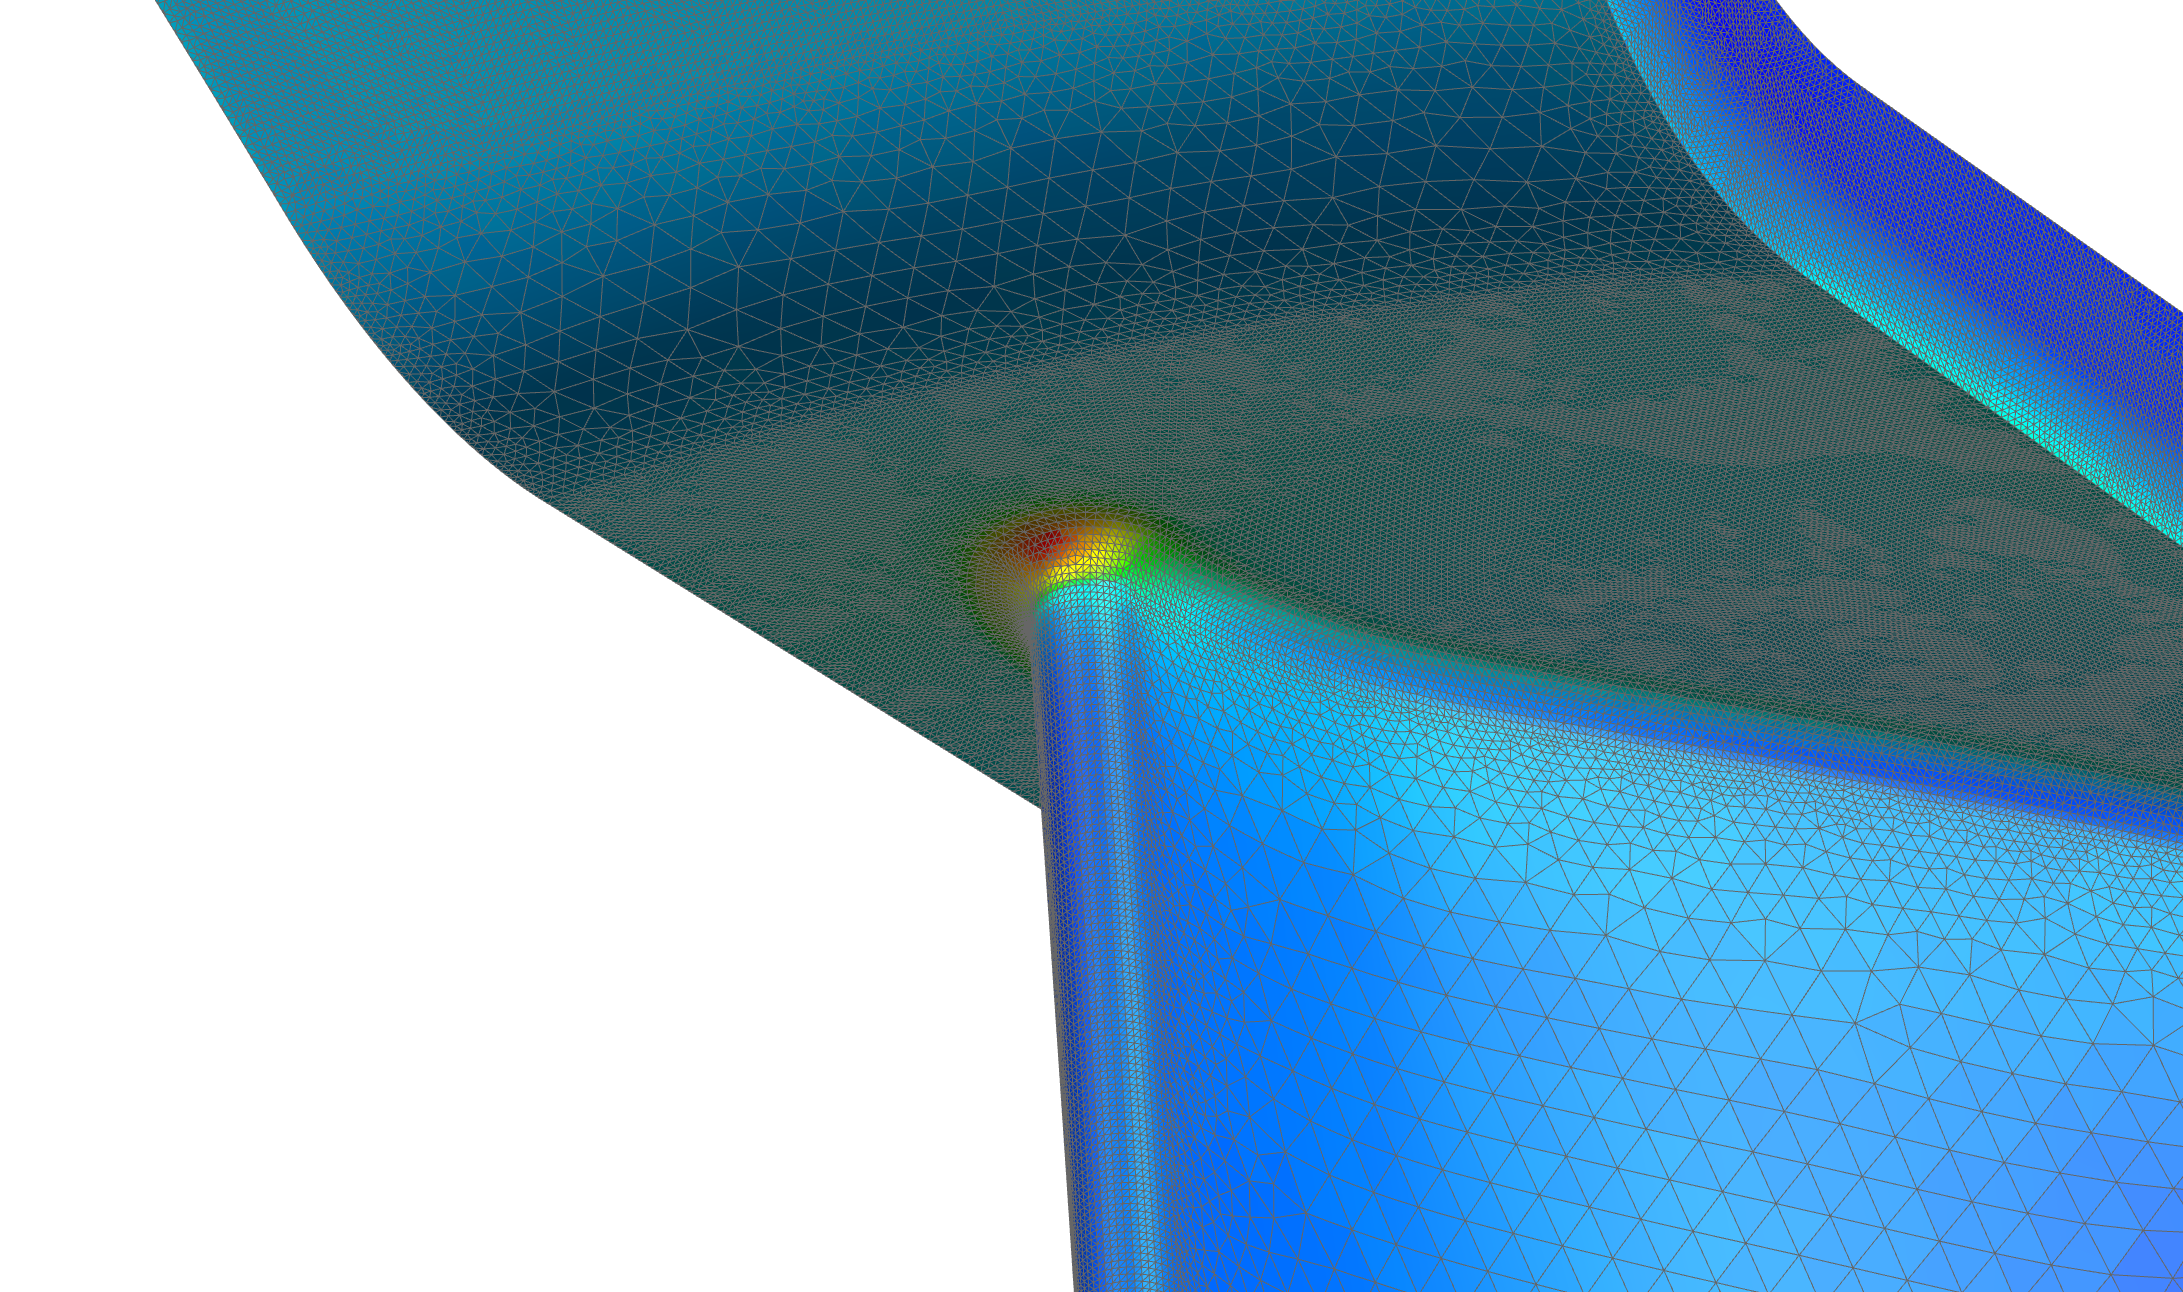
\includegraphics[width=0.8\linewidth]{Figures/stator_shutdown.png}
% 	\caption{Maximum stress during shut-down condition}
%    \label{stator1}
% \end{figure}

\newpage
\section{Battery selection}
\label{Chap:Battery_Selection}
In the current Solar Jet project, the Schübeler 7800 HDME battery has been chosen as the energy carrier unit. A detailed argumentation is lacking however. In this section therefore it is investigated what the battery requirements are for the set goal of the project. A battery selection process will then finally decide upon a suitable battery.
\subsection{Requirements}
\begin{enumerate}
\item Energy\\
The Solar Jet project's short term goal is to set a speed of 450\textit{km/u}. In a previous bachelor thesis of Jasper Oranje \cite{BEP_Jasper} it is noted that this speed is only achievable for a short amount of time because of the EDF heating up. For the energy required, it is then assumed that the Solar Jet has to be able to fly at a cruising speed of 394\textit{km/u} for up to three minutes. With an energy transmission efficiency of 0.7, it is now calculated that the battery needs 547.22\textit{Wh}. This only accounts for overcoming the drag force, and does not take into account the energy needed for acceleration.\\
For the EDF to thrust full power, it draws around 9000\textit{W} and requires a voltage of approximately 50\textit{V}. The current draw can now be calculated from equation \ref{Eq:current_draw}.
\begin{equation}
\label{Eq:current_draw}
I = \frac{P}{V} = \frac{9000}{50} = 180 \textit{A}
\end{equation}
With this, the voltage, the current and the capacity needed have been determined.
\item Safety\\
Lithium-ion batteries are vulnerable to safety issues and can violently decompose when these are not met. The battery should therefore never exceed safety margins set by the manufacturer, which usually include a thermal operating range, a voltage operating range and a maximal charge and discharge current as described in section \ref{Chap:Battery_Safety}.\\
Furthermore the battery should be able to handle crashes. Especially with pouch cells, a construction has to be created to handle mechanical impact preventing internal short-circuit, since a hard-metal casing is non-present.
\item Other\\
Lastly, there are three more aspects. The battery should be as light as possible, as every addition of weight requires more thrust to accelerate. Besides weight, the battery should be dimensioned proportionally so that it fits in the allocated design space. Finally, the battery must be practical: The battery has to be easily removable from the Solar Jet for charging or inspection. The battery assembly from the individual cells must be manageable as well.
\end{enumerate}
\subsubsection{Cylindrical versus Pouch}
The first decision to make is whether to use cylindrical cells or pouch cells. Cylindrical cells come with safety, but also come with complexity, weight and volume. Pouch cells on the other hand come with energy density and relative simplicity, but might be prone to failure.

\textit{Cylindrical cell battery pack}\\
Cylindrical lithium-ion cells come in several sizes, but the 18650 size is almost exclusively used. 18650 stands for 18\textit{mm} in diameter, and 650\textit{mm} in length. Since the size is standardized, the range of options shrinks dramatically. There is only a few select creditable manufacturers and only a few select of chemistries to choose from. To further decrease this list of viable options, the influence of energy requirements has to be checked. 18650 cells always have a nominal voltage of 3.6\textit{V}. This means 14 battery packages in series for the required 50\textit{V} voltage. For the current, 180\textit{A} is needed for the EDF. 18650 batteries can not handle currents of 180\textit{A}, and thus need to be switched in parallel. The amount depends on the maximal current one cell is able to handle. In table \ref{Table:18650_cell_comparison} three option are listed plus an additional battery. Battery info comes from Batterybro \cite{Batterybro}, a 18650 cell vendor that sells top brand batteries, include the manufacturers spreadsheet and rate the batteries themselves aswell to correct for 'enthusiastic' spreadsheets.
\begin{table}[H]
\centering
\caption{18650 cell package needed for 50\textit{V}, 180\textit{A}}
\label{Table:18650_cell_comparison}
\begin{tabular}{|l|l|l|l|l|l|}
\hline
Battery & Current(\textit{A}) & Capacity(\textit{Ah}) & Package & Total capacity(\textit{Wh}) & Total weight(\textit{kg}) \\
\hline\hline
1. Sony VTC4			& 30			& 2							& 14S6P  & 604.8 & 3.780\\ \hline
2. LG Chem HB6			& 30				& 1.5				    & 14S6P & 453.6 & 4.032	 \\ \hline
3. Samsung INR-25R5			& 20			& 2.5			    & 14S9P & 1134 & 5.670\\ \hline
4. Panasonic NCR-B			& 5			& 3.4			    & 14S36P & 6168.96 & 22.780\\ \hline
\end{tabular}
\end{table} 

\subsection{Selecting a battery}
\label{Selecting_A_Battery}

%\begin{figure} [H]
% 	\centering
% 	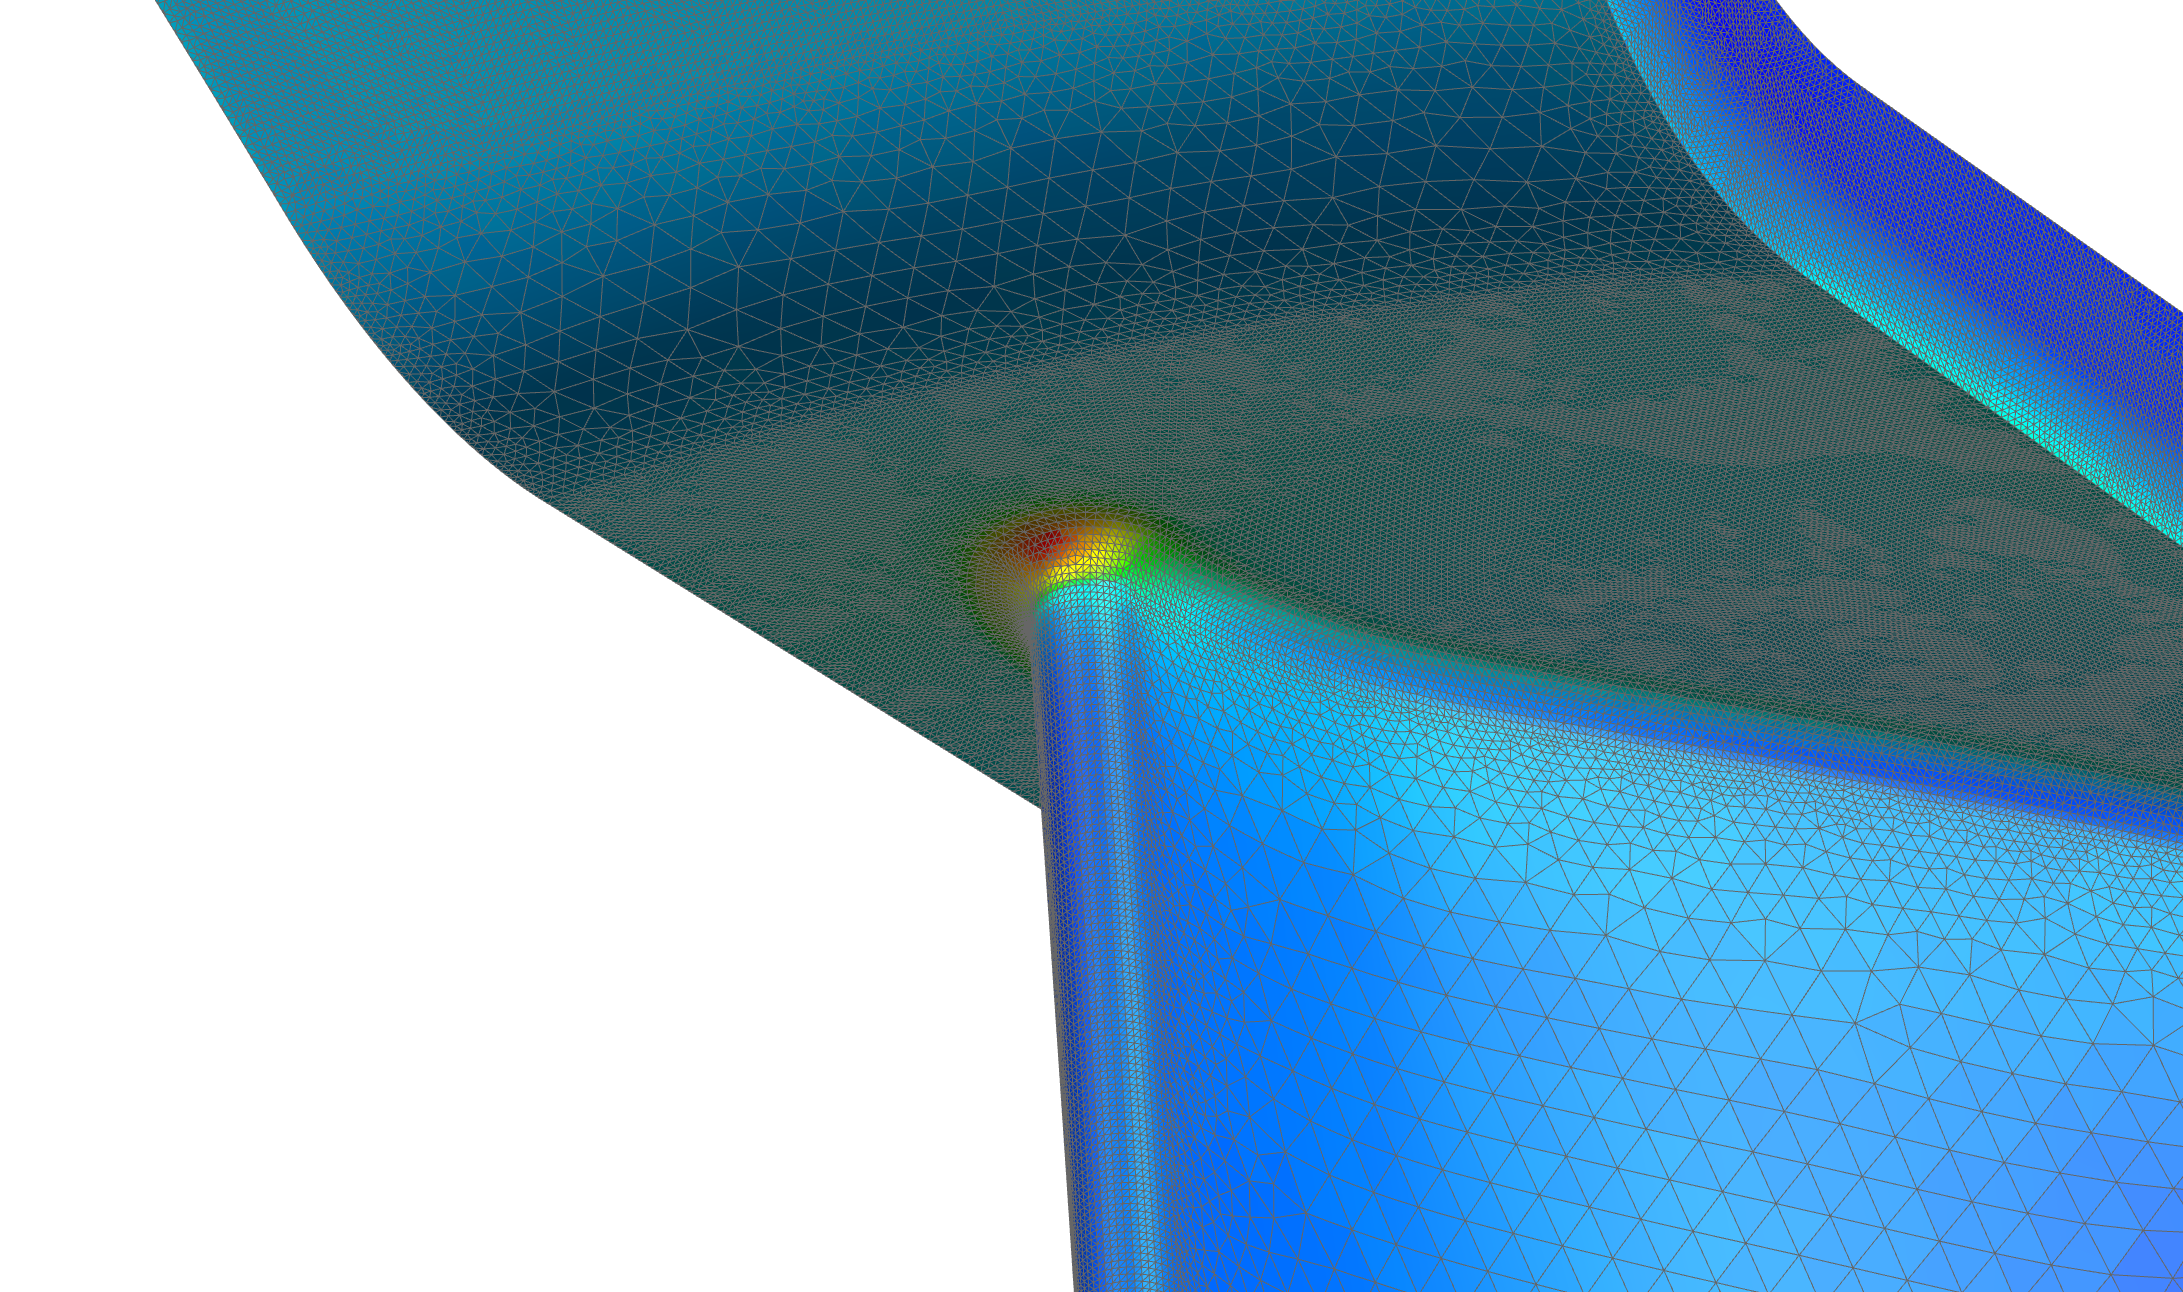
\includegraphics[width=0.8\linewidth]{Figures/stator_shutdown.png}
% 	\caption{Maximum stress during shut-down condition}
%    \label{stator1}
% \end{figure}

\newpage
\section{Thermal Model}
\label{Chap:thermal_model}
\textit{Problem introduction}\\
For the battery to be correctly implemented in the Solar Jet, there are a set of regulations to follow to ensure battery safety and to maximize both lifespan and conservation of its performance. In chapter \ref{Chap:Battery_Safety} these are explained in detail. In section \ref{Sub:Thermal_Stability} thermal specific regulations are set. To verify the batteries in the Solar Jet comply with these specifications, a thermal model is made.

Note that in a previous bachelor thesis \cite{BEP_Rutger}, a thermal measurement was done for the battery as well as for the EDF motor. In this experiment, the EDF was set to maximal power. The speed of power increase was however varied. The results can be seen in figure \ref{Rutger_experiment}.

\begin{figure}[H]
  \centering
  \subfloat[Temperature of the Schubeler 7800HDME 14S1P.]{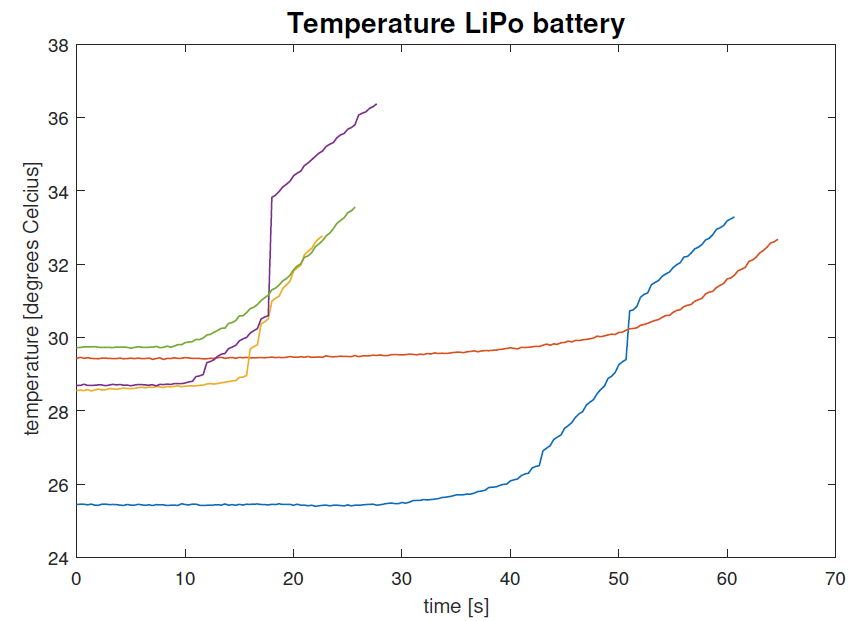
\includegraphics[width=0.5\textwidth]{Figures/Temperature_Battery.PNG}\label{fig:f1}}
  \hfill
  \subfloat[Temperature of the EDF motor.]{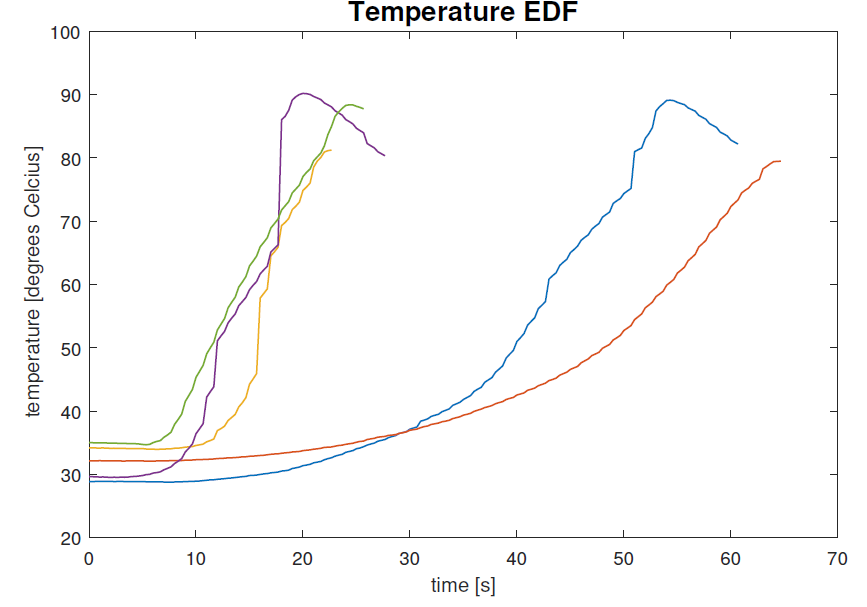
\includegraphics[width=0.5\textwidth]{Figures/Temperature_Motor.PNG}\label{fig:f2}}
  \caption{Temperature measurement of varying power increments to maximal power.}
  \label{Rutger_experiment}
\end{figure}

Degenhart concluded that the batteries did not need active cooling, even when 6 cells are closely packed as they are in the current setup. This because the temperature of the EDF got near its specified maximal temperature faster than the Schübeler 7800HDME LiPo battery did. The incentive to make a thermal model thus seems minimal. However there is two things to consider. 

The first is that the thermocouple used was wedged a little into the side of the battery pack. This can be seen in figure \ref{Thermocouple}. 

\begin{figure} [H]
	\centering
	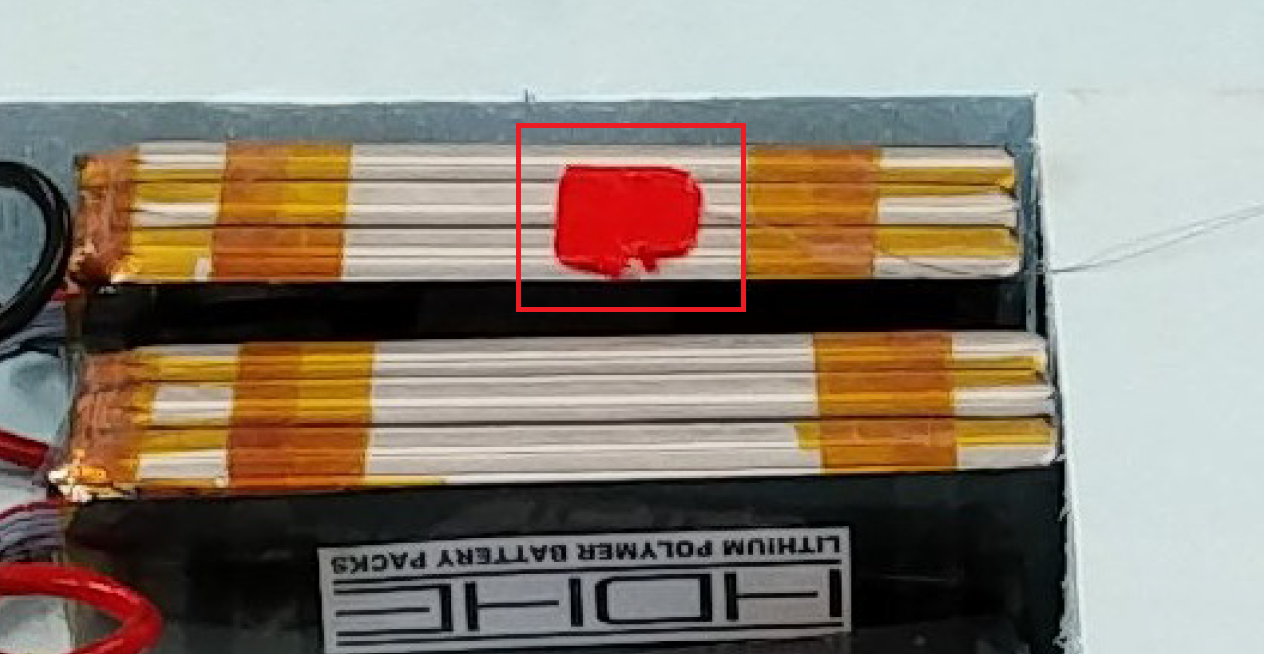
\includegraphics[width=0.5\linewidth]{Figures/Thermocouple.PNG}
	\caption{Thermocouple wedged into the side of the battery}
   \label{Thermocouple}
\end{figure}

The problem with this is that the center of the battery pack will likely get the hottest, whereas now the this is not measured. Another problem is that it measures the temperature of the aluminum foil which is designed to dissipate heat generated by the cells. This means that the inside of a cell might be considerably hotter.

The second incentive is that with a thermal model, it can be analyzed how different variables influence battery thermal behavior. For future designs decisions, the battery thermal behavior would maybe be more influential than it is now. This thermal model can provide data backed arguments for choosing new batteries or implementation decisions such as active cooling or pack design.

The model is used in this bachelor final thesis to question the viability of using a 6S1P battery pack used currently. This is because during the project, one of the 6S1P battery packs had malfunctioned. It was described that the battery was swollen and smelled badly. Swelling is a sign of overheating of the battery as described in section \ref{Chap:Battery_Safety}. It is wondered if a 6S1P maybe is ineffective in losing its heat fast enough. Maybe a less densely packed battery should be used. The model setup is explained, after which an analysis is done comparing the model to the measurements of Degenhart. Finally an example is given of how this model can be used aside from this bachelor thesis.

\subsection{Setting up the model}
\textit{Geometry}\newline
The model is created in 'Comsol Multiphysics 5.2' using the 'Heat Transfer in Solids' module. First, the Melasta SLPB9564159 selected in section \ref{Selecting_A_Battery} is geometrically modeled. The geometry is consisting out of the main battery body and two connection tabs. The aluminum pouch is not geometrically modeled, this is implemented later.

\textit{Material}\newline
Next, a material is assigned to each component. The anode and cathode current collector tabs got assigned aluminum and copper respectively. The material properties in Comsol provide all the required constants for the equations used for the tabs. 
Now for the battery cell however, a material can not be assigned as easily. The lithium-ion battery cell consists out many stacked alternating layers of different materials. Therefore the parameters used in the calculations have to be estimated and assigned manually for the cell component. The final properties used for all components can be seen in table \ref{Table:Material_Properties}.

\begin{table}[H]
\centering
\caption{Material properties}
\label{Table:Material_Properties}
\begin{tabular}{|l|l|l|l|l|}
\hline
Property & Anode & Cathode & Battery & Unit                   \\ \hline \hline
$C_p$       & 900   & 385     & 800     & J/(kg$\cdot$K)               \\
$\rho$      & 2700  & 8960    & 2129    & kg/m\textsuperscript{3} \\
$k$        & 238   & 400     & 30$\vec{e}_{xx}$, 30$\vec{e}_{yy}$, 0.3$\vec{e}_{zz}$      & W/(m$\cdot$K)            	  \\ \hline   
\end{tabular}
\end{table}

Thus for the cell there are three properties to be determined: The specific heat capacity $C_p$, the density $\rho$ and the thermal conductivity $k$. The properties are determined by assuming the cell as a homogeneous material that averages the properties of the real materials (taking into account the amount of each material). The problem is that for every battery the amount of material, and the material used is different. 

\textit{Density}\newline
The data sheet \textbf{REFEREREN NAAR DATASHEET IN APPENDIX} for the Melasta SLPB9564159 provides both the dimensions and weight of the battery. The density can thus be calculated by formula \ref{Eq:density}.

\begin{equation}
\label{Eq:density}
\rho = \frac{m}{l\cdot h \cdot w} = \frac{0.201}{0.159\cdot 0.065 \cdot 0.0095} = 2128.7 \quad (kg/m^3)
\end{equation}

\textit{Specific heat capacity and thermal conductivity}\newline
For the selected Melasta battery these are not provided in the data sheet, thus  constraining $C_p$ and $k$ to be determined from literature since the chosen cell is not available for measurements. Different sources cite different values, especially for the specific heat capacity, as seen in table \ref{Table:Specific_heat_thermal_conductivity}. 

\begin{table}[H]
\centering
\caption{Specific heat capacity from different sources}
\label{Table:Specific_heat_thermal_conductivity}
\begin{tabular}{|l|l|l|}
\hline
Source & $C_p$ [J/(kg$\cdot$K] & Chemistry                    \\ \hline \hline
\cite{Ahmad}       & 800   & Unknown                     \\
\cite{Kirill_Murashko}(p82)       & 1000   & LTO               	  \\
\cite{W.}       & 1243   & LMO               	  \\
\cite{Nur}       & 1300   & LFePO               	  \\
\hline   
\end{tabular}
\end{table}

It can be seen that this varies quite a bit. The chosen value is 800 [J/kg$\cdot$K] for $C_p$. The chemistry is important here. LFePO, LTO and LMO Lithium-ion batteries are often used in high temperature applications because of their high $C_p$. This can also be concluded from the thermal runaway section \ref{Sub:Thermal_Stability}, whereas LCO usually has a lower $C_p$ and is arguably the least thermally stable chemistry \cite{Kirill_Murashko}(p31) \cite{types_of_batteries}.\\ It is unfortunate however that no study was found that specifically determined the LCO heat capacity used in most commercially available pouch cells (and in the Melasta cells). \newline
For the thermal conductivity it is specified in sources that this is averagely 30 [W/m$\cdot$K] in-plane, and a factor 100 less out-of-plane \cite{Kirill_Murashko}\cite{W.}. This anisotropic behavior originates from the stacked alternating layer design of a pouch cell where the metal current collectors conduct well, whereas the in-between material conducts worse. A multilayer insulator is thus formed out-of-plane \cite{MLI}. The effect can be calculated by formula \ref{Eq:thermal_conductivity}.

\begin{equation}
\label{Eq:thermal_conductivity}
\frac{\delta}{k} = \frac{\delta_1}{k_1} + \frac{\delta_2}{k_2} + ... +\frac{\delta_n}{k_n}
\end{equation}

where $\delta$ is the layer thickness [m], and $k$ the thermal conductivity [W/m$\cdot$K]. \\When this is applied to the battery, the in-plane $k$ is determined by only one battery layer for its whole plane. Whereas out-of-plane $k$ is determined by a hundred fold times this battery layer, with each battery layer decreasing the average thermal conductivity.

\textit{Load conditions}\newline
With now both the geometry and the material properties assigned. Finally the load conditions have to be applied. Comsol will then be able to solve the heat equation given by formula \ref{Eq:heat_equation}.
\begin{equation}
\label{Eq:heat_equation}
\rho C_p \dfrac{\partial T}{\partial t} - \nabla \cdot (k\nabla T) = \dot{q}
\end{equation}
Boundary conditions, initial conditions and constants need to be assigned for the model to solve the heat equation:
\begin{enumerate}
\item First the initial temperature is defined as 298 [K] resembling room temperature and the temperature used in the before mentioned bachelor thesis. 
\item Then the material properties of table \ref{Table:Material_Properties} are applied to their domains.
\item A thin layer condition is then applied on all battery cell sides to simulate the aluminum pouch circumventing the battery. This is illustrated in figure \ref{thinlayer}, where blue indicates the domain. Not seen is that between the cells the layer condition is applied as well (indicated with red). The material properties assigned to the foil are the same as for the anode current collector, as they are both aluminum.
\begin{figure} [H]
	\centering
	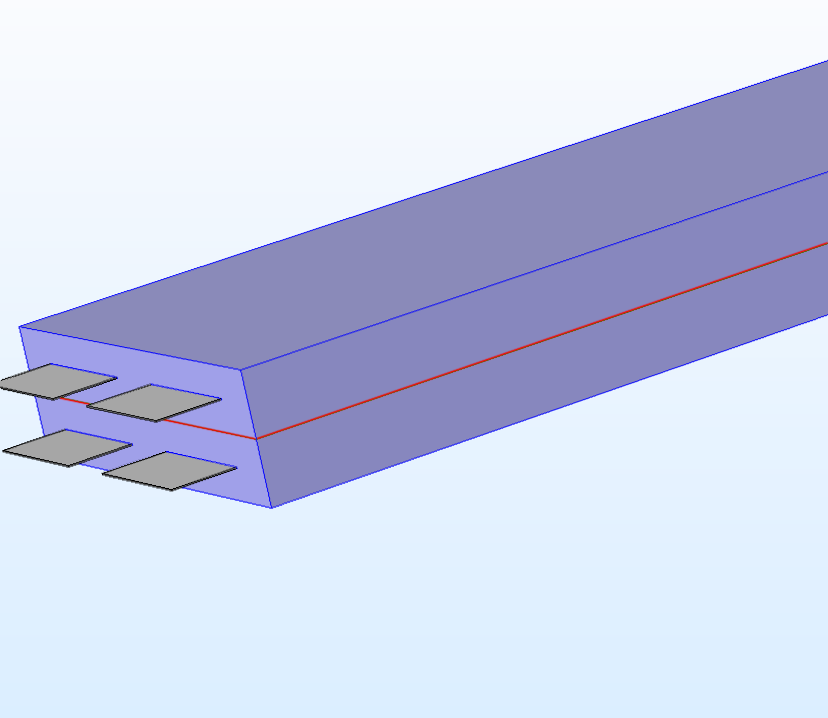
\includegraphics[width=0.5\linewidth]{Figures/thinlayer.png}
	\caption{Domain on which the aluminum layer is applied.}
   \label{thinlayer}
\end{figure}
\item Convection is then simulated by adding a convective boundary condition at all outer faces of the battery. This includes the tabs, but excludes the surface between cells. An ambient temperature of 298 [K] is set. For non-moving air a convection coefficient of $h = 10$ [W/m$^2 \cdot$K] is assumed initially \cite{heat_transfer_coefficient}. 
\item Finally, heat generation has to be simulated. An internal heat source is set per domain by calculating joule heating from formula \ref{Eq:joule_heating}.

\begin{equation}
\label{Eq:joule_heating}
\dot{q} = \frac{P}{V}
\end{equation}

With $\dot{q}$ the heat generated per volume [W/m$^3$], $P$ the power [W], $V$ the volume [m$^3$]. The volume of both the tab and cell domain can be calculated by the given dimensions from the Melasta datasheet.\\
For the power generated by the tab domains, formula \ref{Eq:tab} is used.
\begin{equation}
\label{Eq:tab}
P=R'I^2 \quad ;\quad R'=\rho'\frac{L}{A}
\end{equation}
With $I$ being the current [A], $R'$ being the electrical resistance [$\ohm$], $R$ being the electrical resistivity [$\ohm \cdot$ m], $A$ the cross sectional area the current is flowing through [m$^2$] and $L$ the length of the area the current is flowing through [m]. The $\rho'$ of aluminium is $2.65\cdot 10^-8$ [$\ohm\cdot$ m] and that of copper is $1.68\cdot 10^-8$ [$\ohm\cdot$ m]. This means that the aluminum tab will be hotter since the resistance is higher, and both tabs are the same size (specified by the Melasta Datasheet). \\
Then for the cell domain formula \ref{Eq:cell_not_used} should be used.
\begin{equation}
\label{Eq:cell_not_used}
P=RI^2+(T[\frac{dE}{dT}])I
\end{equation}
However, the most right hand term, the internal entropy change, has to be measured and has minor impact compared to the first right hand term. This entropy change is thus neglected, leaving us with the same formula as for the tab domain, formula \ref{Eq:tab}. We do not need to calculate $R$ by the resistivity formula since $R$ is given by the Melasta Datasheet ($R = 2\cdot 10^-3$) [$\ohm$]. \\
$I$ is chosen to be 180 [A] since this was drawn by the EDF motor in the previous bachelor thesis, as seen in figure \ref{Fig:Typical_Current}.
\begin{figure} [H]
	\centering
	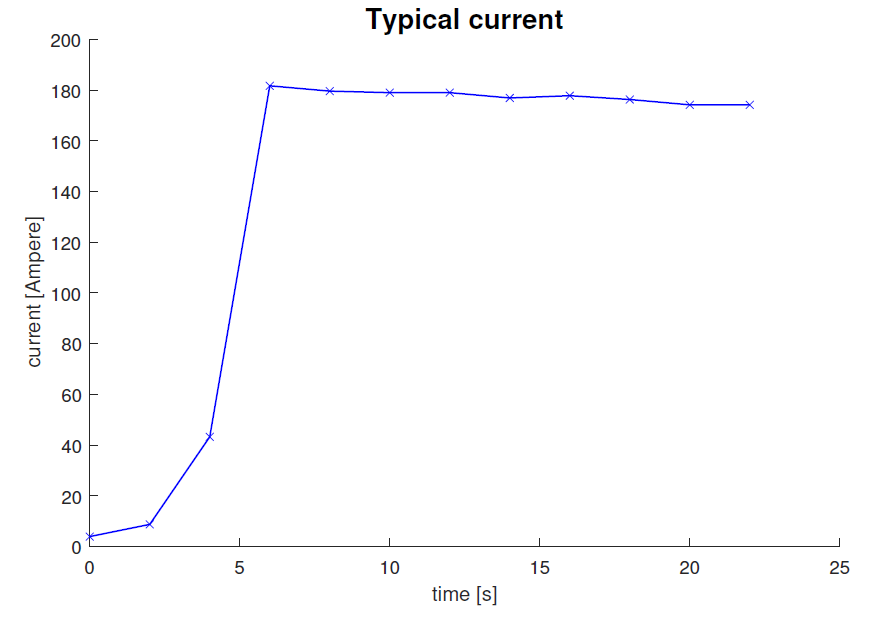
\includegraphics[width=0.5\linewidth]{Figures/Typical_Current.PNG}
	\caption{Current measured on EDF full throttle.}
   \label{Fig:Typical_Current}
\end{figure}
\end{enumerate}
The model has now been completed and can be run. Again, it is opted to test whether it is viable for the Solar Jet to use a 6S1P battery pack. A 1S1P pack will be modeled, as well as a 6S1P pack, after which the results are compared.\\ \newline
The model is then validated in \ref{Sub:Validation}.



\subsection{Results}
With the model set up, it is analyzed how the simulation behaves and if the results are intuitive. Then it is checked whether the results compare to the results gotten from Degenhart his measurements. Finally the difference between a 6S1P and a 1S1P battery pack is analyzed.

\textit{6S1P Battery pack}\\
The model for the 6S1P is simulated for 300 seconds. The thermal results are then analyzed both spatially and as function of time. The thermal image of the battery after 300 seconds can be seen in figure \ref{Fig:thermal_image}. A thermal image of 60 seconds is also displayed, as 60 seconds is a more realistic flight time.

\begin{figure}[H]
  \centering
  \subfloat[Thermal image at 60 seconds.]{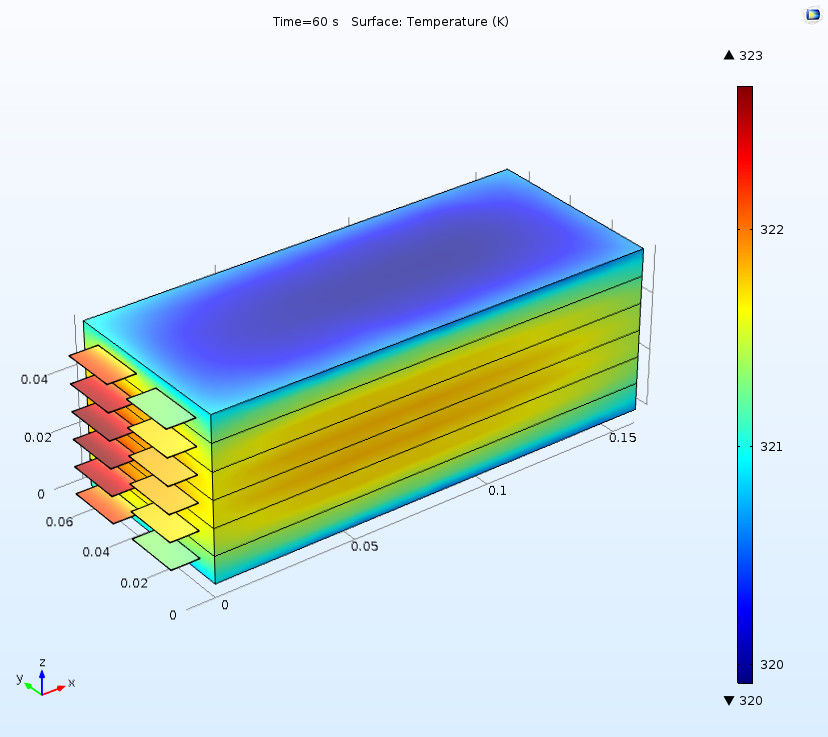
\includegraphics[width=0.5\textwidth]{Figures/6_thermal.png}\label{Fig:6_thermal_image_60s}}
  \hfill
  \subfloat[Thermal image at 300 seconds.]{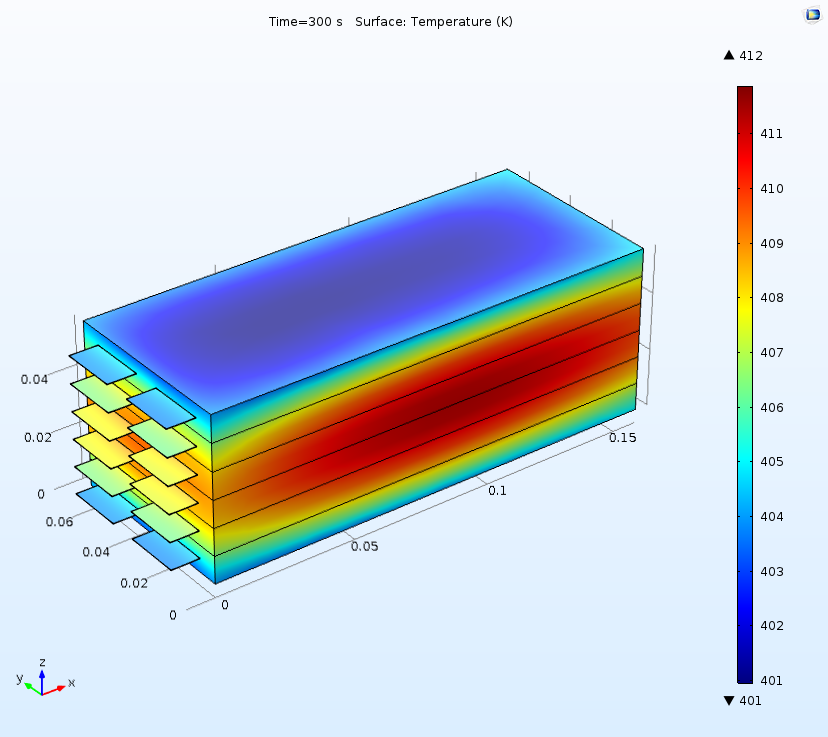
\includegraphics[width=0.5\textwidth]{Figures/6_thermal_300s.png}\label{Fig:6_thermal_image_300s}}
  \caption{Thermal image.}
  \label{Fig:thermal_image}
\end{figure}

It is seen that as expected, the core is the warmest in the battery, and that the top and bottom surfaces are coolest because of the anisotropic thermal conductivity. Note however that the middle area of the top surface has a slightly lower temperature than the top surface edges. This is strange intuitively, but is explained by the aluminum pouch surrounding the battery. With its high thermal conductivity it transfers some of the heat of the side surfaces to the cooler top surface. Note that for 60 seconds, the hottest parts are the anodes of the battery, caused by the small cross-sectional area the current passes through. A bus bar should be designed to diminish or at least cope with this temperatures.

The temperature is now analyzed both spatially and as function of time. In Comsol, a point or line in 3D can be assigned of which the temperature values can then be plotted. For the spatial analyses a line is defined from the bottom to the top surface at the middle of the battery as seen in Appendix \ref{Fig:6_4}. For the transient analysis, a point is defined. The point is chosen to be located in the middle of the third battery, the critical temperature location as can be see in figures \ref{Fig:6_1} and \ref{Fig:6_2}. Since the problem is symmetric the point could also have been chosen in the fourth battery. Note however that between the two batteries, in the middle of the pack the temperature is actually lower because of the aluminum pouch. The chosen point is presumed hottest, however the hottest point is actually shifting as a function of time: The current collector tabs warm up relatively fast compared to the battery at first, however as time progresses the battery grows hotter thus shifting the point more to the batteries center.

The spatial result can be seen in figure \ref{Fig:Out_Of_Plane_300s}. As stated above, the problem is symmetric vertically and as expected the critical temperature is located in the middle two batteries. The effect of the aluminum pouch is clearly seen here. In the appendix figure \ref{Fig:6_5} is included showing the temperature distribution without aluminum foil. It can be seen that the maximum temperature is higher and is more lumped. Clearly the aluminum foil dissipates energy from the pack.

\begin{figure} [H]
	\centering
	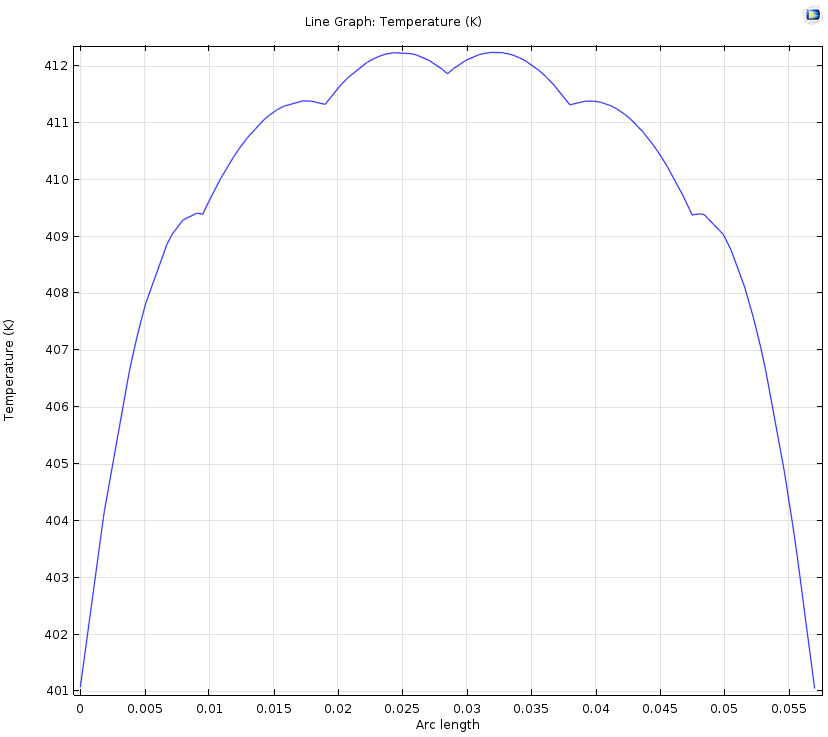
\includegraphics[width=0.5\linewidth]{Figures/300s_10h_180A_2mOhm_OutOfPlaneLast.png}
	\caption{Spatial out of plane thermal analysis at 300 seconds.}
   \label{Fig:Out_Of_Plane_300s}
\end{figure}

The transient result is given in figure \ref{Fig:Transient_10h_300s}. It can be seen that the temperature increases basically linear in the first 300 seconds. This is explained by the low convective heat transfer coefficient. It can be seen that a 6S1P that discharges at 180 [A] for the full 300 seconds will be way overheated with no active convective cooling.

\begin{figure} [H]
	\centering
	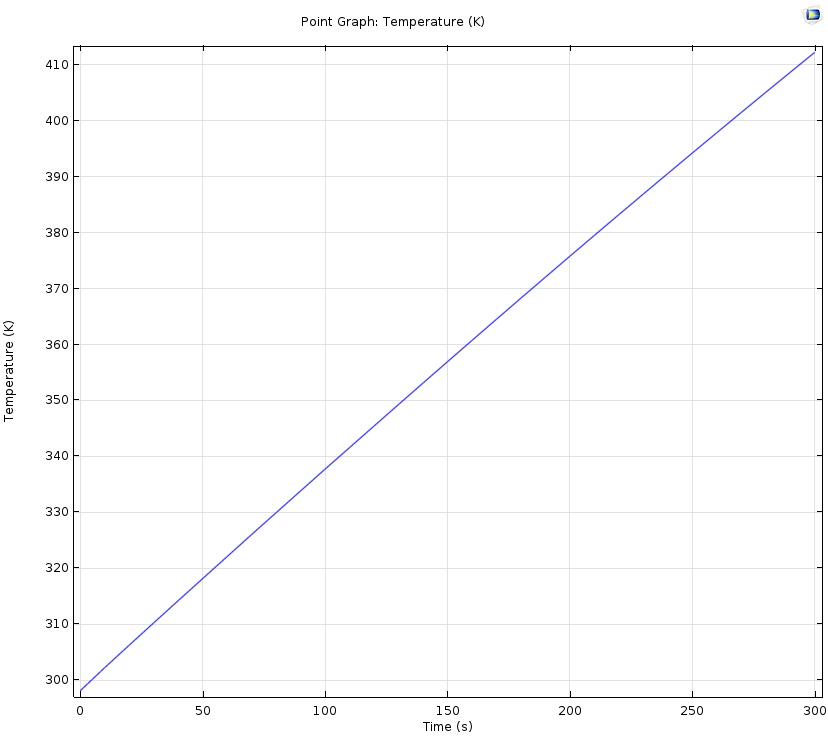
\includegraphics[width=0.5\linewidth]{Figures/300s_10h_180A_2mOhm.png}
	\caption{Transient thermal analysis at 300 seconds.}
   \label{Fig:Transient_10h_300s}
\end{figure}

\textit{Comparing the 6S1P battery simulation with the experiment}\\
Before the 6S1P is compared with the 1S1P pack, it is first checked if the results of the 6S1P model gives similar results to the measurement done in Degenhart his bachelor thesis.

In figure \ref{Rutger_experiment} it is seen that the measurement duration was effectively only 10 to 20 seconds before the EDF got to a critical temperature. In those seconds the temperature of the battery rose as well. The simulation of a 6S1P is compared with these results. In figure \ref{Fig:6_3} the location of measurement in the simulation is seen. This is estimated to be the point as where the real thermocouple was placed. The transient behavior is given in figure \ref{Fig:Transient_10h_60s}.

\begin{figure} [H]
	\centering
	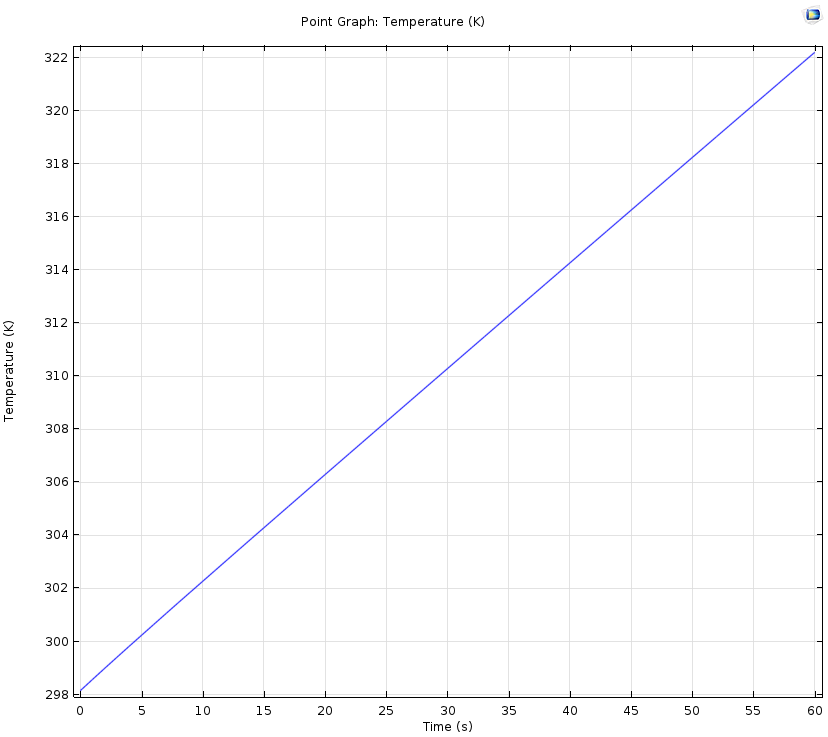
\includegraphics[width=0.5\linewidth]{Figures/60s_10h_180A_2mOhm.png}
	\caption{Transient thermal analysis at 60 seconds at thermocouple location.}
   \label{Fig:Transient_10h_60s}
\end{figure}

When this result is compared to the measurements. The following figure \ref{Fig:Simulation_Measurement_Comparison} is obtained. It is seen that the gradient is a little steeper for the simulation but nearly identical. This slight difference can be caused by the entropy term left out in \ref{Eq:joule_heating} which can be negative. It can also be because of the parameters chosen, like the specif heat capacity $C_p$, or the assumption of the battery being one solid material. However it is concluded the simulated model is acceptably realistic. 

\begin{figure} [H]
	\centering
	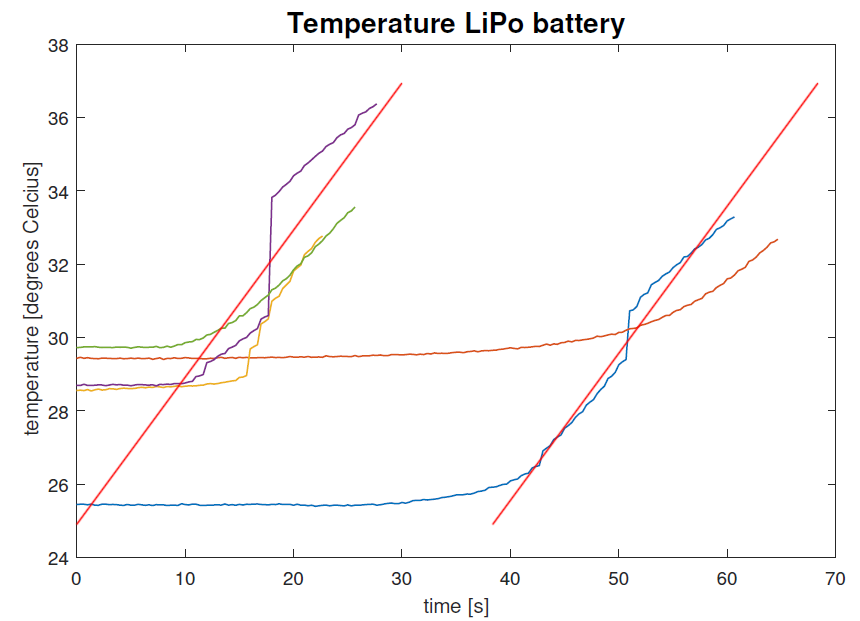
\includegraphics[width=0.5\linewidth]{Figures/Temperature_Battery_Comparison.png}
	\caption{Simulation compared to measurement results}
   \label{Fig:Simulation_Measurement_Comparison}
\end{figure}

\textit{Comparing the 6S1P with 1S1P battery}\\
For the 1S1P the same parameters and configurations are used. Also the same sample points and lines are used. It is hypothesized that a 1S1P will show a faster decline in temperature gradient, and thus have a lower maximum temperature. The simulation is again ran for 300 seconds. This gives the result seen in figure \ref{Fig:1_thermal_behavior}. It can be seen that the temperature is indeed lower. An impact of around 25 [K]. However, in the first 60 seconds, the temperature is almost exactly the same. For the current flight setup, it should therefore not matter if a 6S1P or a 1S1P battery is used. This was already concluded by Degenhart his bachelor thesis and thus is not that of a surprising result.

\begin{figure}[H]
  \centering
  \subfloat[Transient behavior 1S1P 300 seconds.]{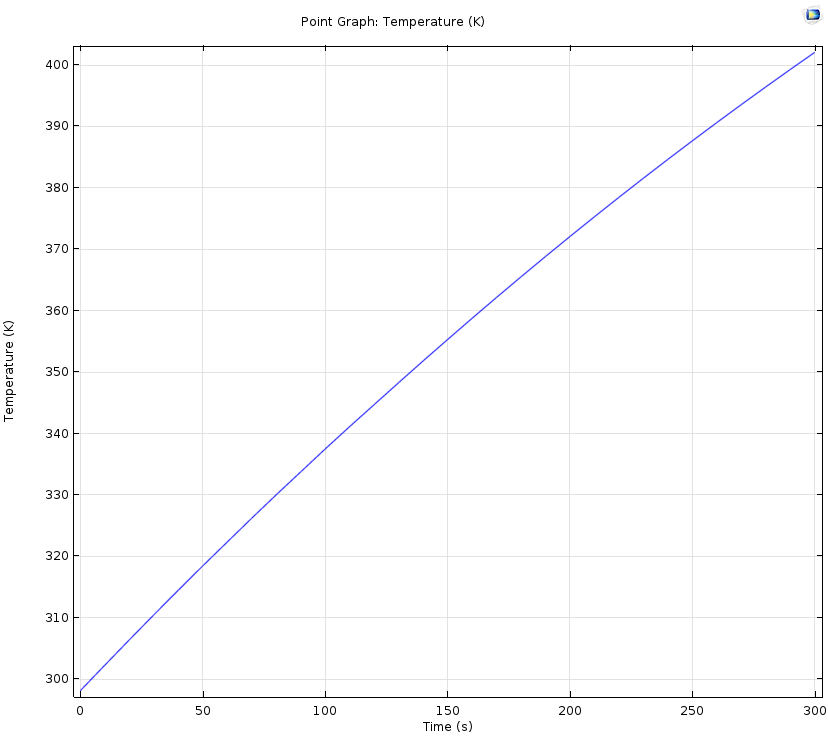
\includegraphics[width=0.5\textwidth]{Figures/1_300s_10h_180A_2mOhm.png}\label{Fig:1_transient_300s}}
  \hfill
  \subfloat[Spatical behavior 1S1P 300 seconds.]{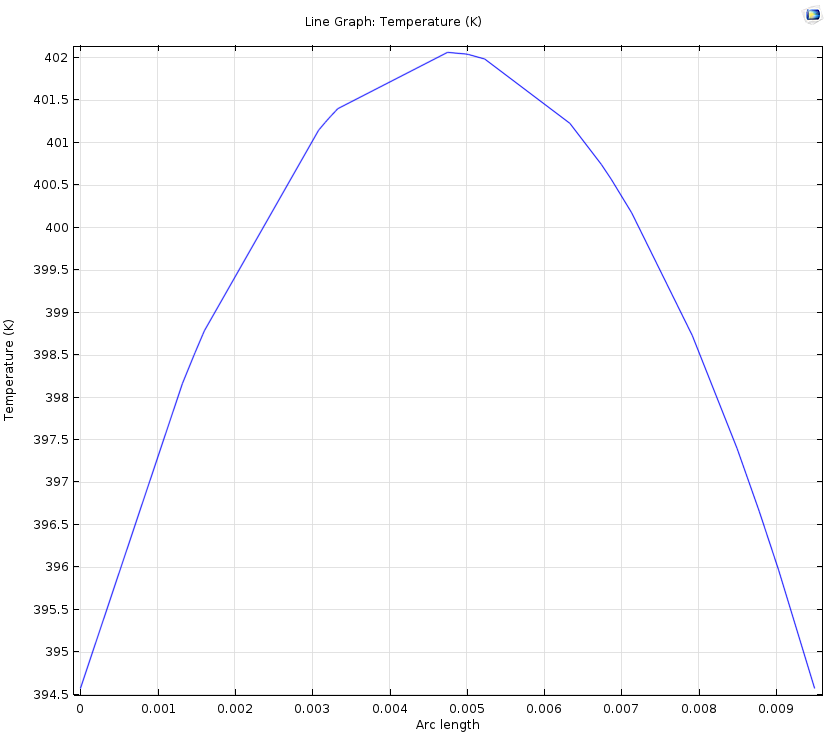
\includegraphics[width=0.5\textwidth]{Figures/1_300s_10h_180A_2mOhm_OutPlaneLast.png}\label{Fig:1_spatial_300s}}
  \caption{Thermal behavior at 300 seconds.}
  \label{Fig:1_thermal_behavior}
\end{figure}

\textit{When does a 1S1P make a difference?}\\
Unlike actual measurements, with this model it is possible to analyze design choices without actually taking the time, effort or costs to set up an experiment. Thus it could be asked, what if the current setup of the Solar Jet is disregarded. What if the motor is now cooled and maximum power is now required for not 20 seconds, but 3 minutes. 3 minutes is assumed to be a desirable flight time at maximal power according to a bachelor thesis of Jasper Oranje \cite{BEP_Jasper}. 

From figure \ref{Fig:1_transient_300s_200h} and \ref{Fig:6_transient_300s_200h} it is clear both do not suffice for a 180 second maximal power flight. For the 6S1P and 1S1P the temperature at 180 seconds is 365 and 368 [K] respectively, whereas their safe operating temperature which it should not exceed is 323 [K]. This means that the batteries need to be cooled. From \cite{heat_transfer_coefficient} it is gotten that $h$ is 100 [W/m$^2$K] for a moderate speed flow of air. When the Solar Jet is flying at maximal power, it is assumed that this speed is high and surrounding air can be channeled to the battery compartment, doubling $h$. If this value of 200 [W/m$^2$K] is really achieved by high speed air flow, is to be measured however. It might seem to be a crude assumption, though this is also chosen for the sake of argument. Because when the model is simulated again with the new heat transfer coefficient of 200 [W/m$^2$K], a satisfying result is obtained: for a 1S1P pack the maximal allowable temperature is just barely reached, see figure \ref{Fig:thermal_behavior_200h}. 

\begin{figure}[H]
  \centering
  \subfloat[Transient behavior 1S1P $h = 200$]{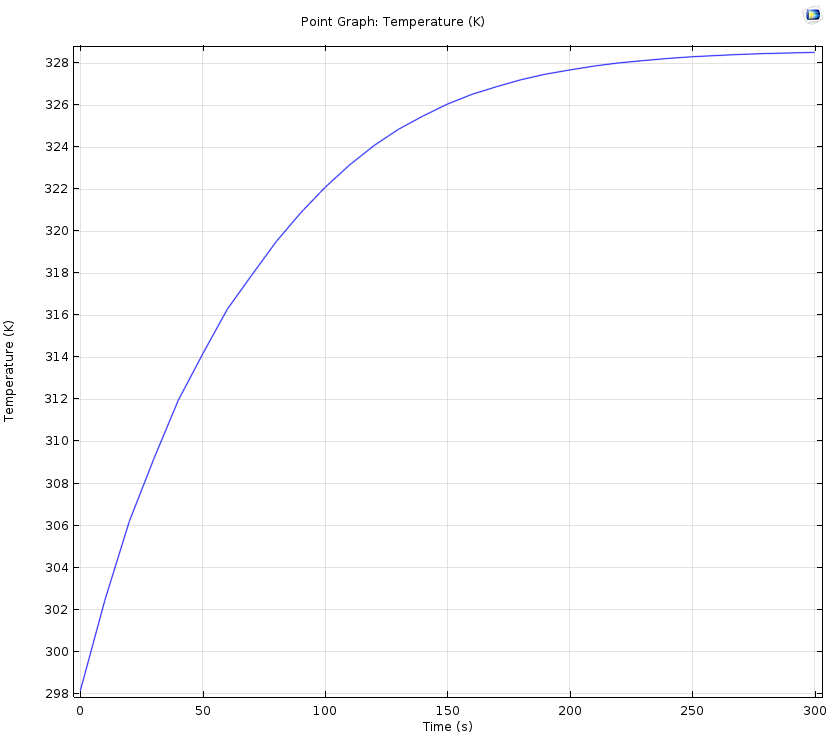
\includegraphics[width=0.5\textwidth]{Figures/1_300s_200h_180A_2mOhm.png}\label{Fig:1_transient_300s_200h}}
  \hfill
  \subfloat[Transient behavior 6S1P $h = 200$]{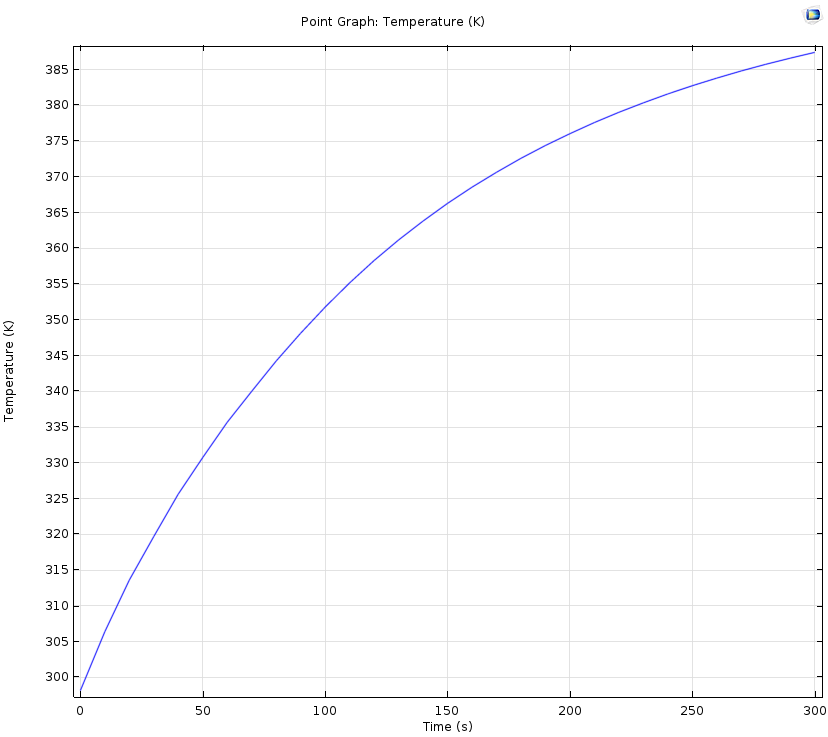
\includegraphics[width=0.5\textwidth]{Figures/300s_200h_180A_2mOhm.png}\label{Fig:6_transient_300s_200h}}
  \caption{Thermal behavior $h = 200$ }
  \label{Fig:thermal_behavior_200h}
\end{figure}

From these results it can be concluded that if high power is required for an extended period of time, adequate cooling is required. From the figures, active cooling with air turns out to be much more effective for single cell configurations.

\textit{Recommendations for further research}\\
Active air cooling like investigated above is one the examples out of many different possibilities to be explored. There is a whole range of possible parameters to be twitched. Changes in dimension or internal resistance can be checked, which comes to mind when choosing a new battery cell. Or should a longer flight be required, but channeling air flow to batteries is aerodynamically too disruptive, choosing for a parallel battery setup can be analyzed since the power draw per cell will be halved. Another option to be investigated in this case is liquid cooling. However this all is not in the scope of this thesis since it is focused on the current set up of the Solar Jet, where thermal battery problems are now determined to be minimal. A final option is incorporate an electrical flow simulation in the battery, to better simulate the heat generation in the battery, for example the surface cooling problem explained in section \ref{Sub:Electrical_Stability}.

\subsection{Validation}
\label{Sub:Validation}
Since for the model the heat equation with heat generation is solved with convective and conductive boundary conditions only,  it is possible to solve this equation analytically in 1D and compare this to the numerical result. A steady-state condition is assumed, which reduces the analytical complexity and can be calculated in Comsol with the steady-state solver as well.

Steady state reduces the heat equation \ref{Eq:heat_equation} to equation \ref{Eq:heat_equation_steady-state}.
\begin{equation}
\label{Eq:heat_equation_steady-state}
\frac{\partial T^2}{\partial ^2 x} = -\frac{\dot{q}}{k}
\end{equation}
When this is integrated, equation \ref{Eq:heat_flux} is gotten that gives the heat flux.
\begin{equation}
\label{Eq:heat_flux}
\frac{\partial T}{\partial x} = -\frac{\dot{q}}{k}x + C_1
\end{equation}
Integrating this again gives the temperature field in the domain given by equation 
\begin{equation}
\label{Eq:temperature_field}
T(x) = - \frac{\dot{q}}{2k}x^2 + C_1 x + C_2
\end{equation}
With $C_1$ and $C_2$ the integration constants.\\
Two boundary conditions ($BC$) are now defined and applied which solves the temperature field \ref{Eq:temperature_field}. $T_{wall}$ being the temperature at the wall surface [K] and L being the distance from the center to the outside surface of the wall [m].
\begin{equation*}
BC_1 \quad T = T_{wall}|_{T(L)} \qquad\qquad BC_2 \quad \frac{\partial T}{\partial x} = 0|_{T(0)} 
\end{equation*}
which results in $C_1 = 0$ and $C_2 = T_{wall}$ and finally gives equation \ref{Eq:final_temperature_field}.
\begin{equation}
\label{Eq:final_temperature_field}
T(x) = \frac{\dot{q}L^2}{2k}(1-\frac{x^2}{L^2})+T_{wall}
\end{equation}
This solves the temperature field if $T_{wall}$ is obtained, which is possible by calculating the heat flux at the wall surface due to conduction and convection.
\begin{equation}
\label{Eq:total_heat_flux}
Q = k\frac{\partial T}{\partial x} = h(T_{wall} - T_{ambient})
\end{equation}
With $Q$ being the heat flux [W] and $T_{ambient}$ the environmental temperature [K]. When substituting \ref{Eq:heat_flux} into \ref{Eq:total_heat_flux}, $T_{wall}$ can now be calculated:
\begin{equation}
T_{wall} = \frac{\dot{q}L}{h}+T_{ambient}
\end{equation}
Which gives the final temperature field equation \ref{Eq:final_temperature_field2}.
\begin{equation}
\label{Eq:final_temperature_field2}
T(x) = \frac{\dot{q}L^2}{2k}(1-\frac{x^2}{L^2})+\frac{\dot{q}L}{h}+T_{ambient}
\end{equation}

The temperature field is calculated in matlab making sure the same parameters are used as in Comsol. For $h = 10$, $k = 0.3$, $\dot{q} = 180^2 \exp^-3$ and $L = 0.0095/2$ (parameters used for the battery out-of-plane) the results gotten are plotted in figure \ref{Fig:Comparison}. It is seen that the results match almost perfectly. It is concluded Comsol calculates the conductive and convective conditions accurately.

\begin{figure}[H]
  \centering
  \subfloat[Numerical result Comsol.]{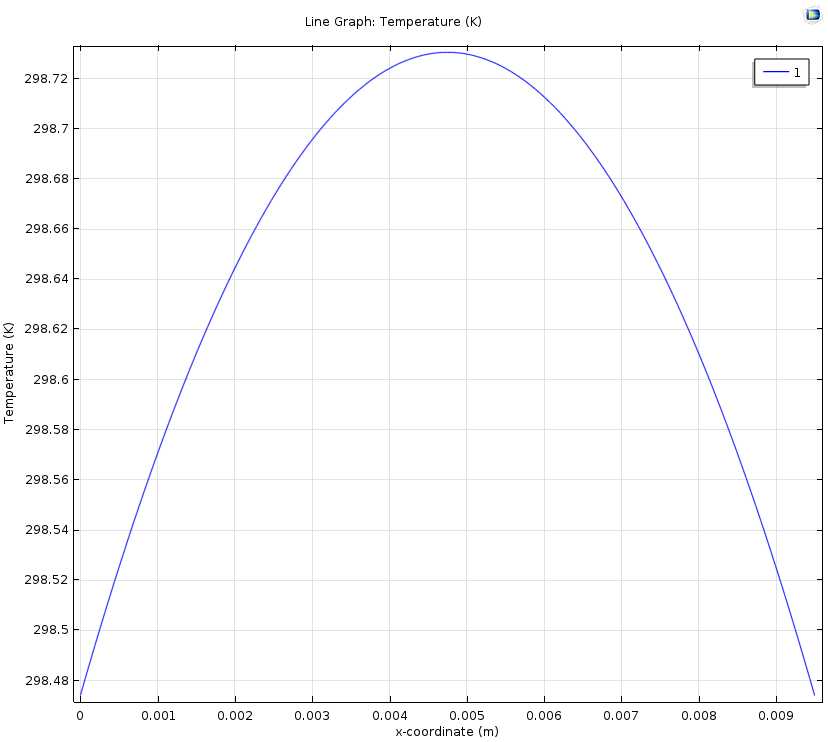
\includegraphics[width=0.5\textwidth]{Figures/comsol_analytical.png}\label{Fig:comsol_analytical}}
  \hfill
  \subfloat[Analytical result Matlab.]{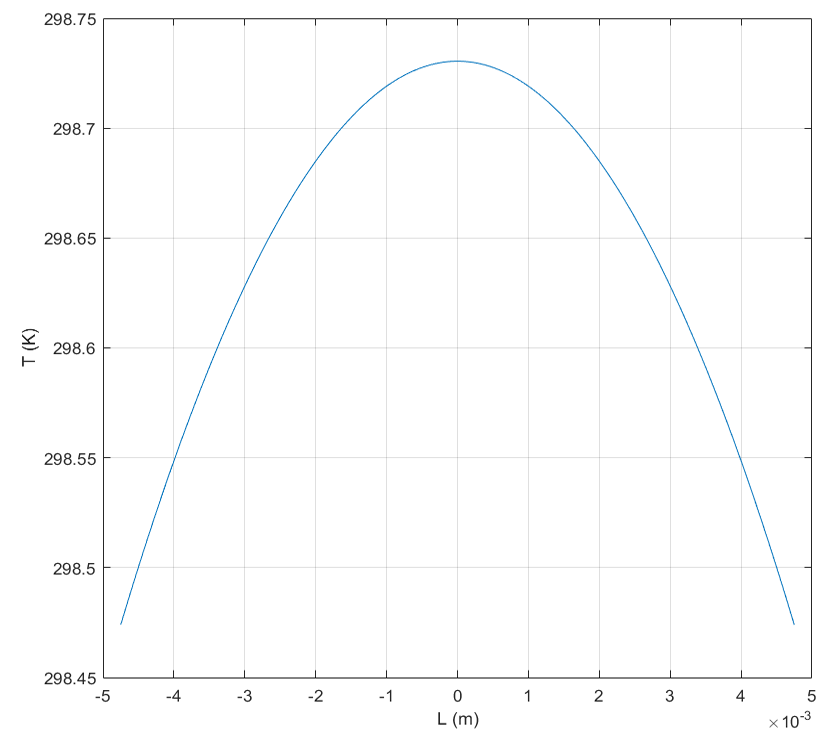
\includegraphics[width=0.5\textwidth]{Figures/matlab.png}\label{Fig:matlab_analytical}}
  \caption{Comparison numerical versus analytical.}
  \label{Fig:Comparison}
\end{figure}









%\begin{figure} [H]
% 	\centering
% 	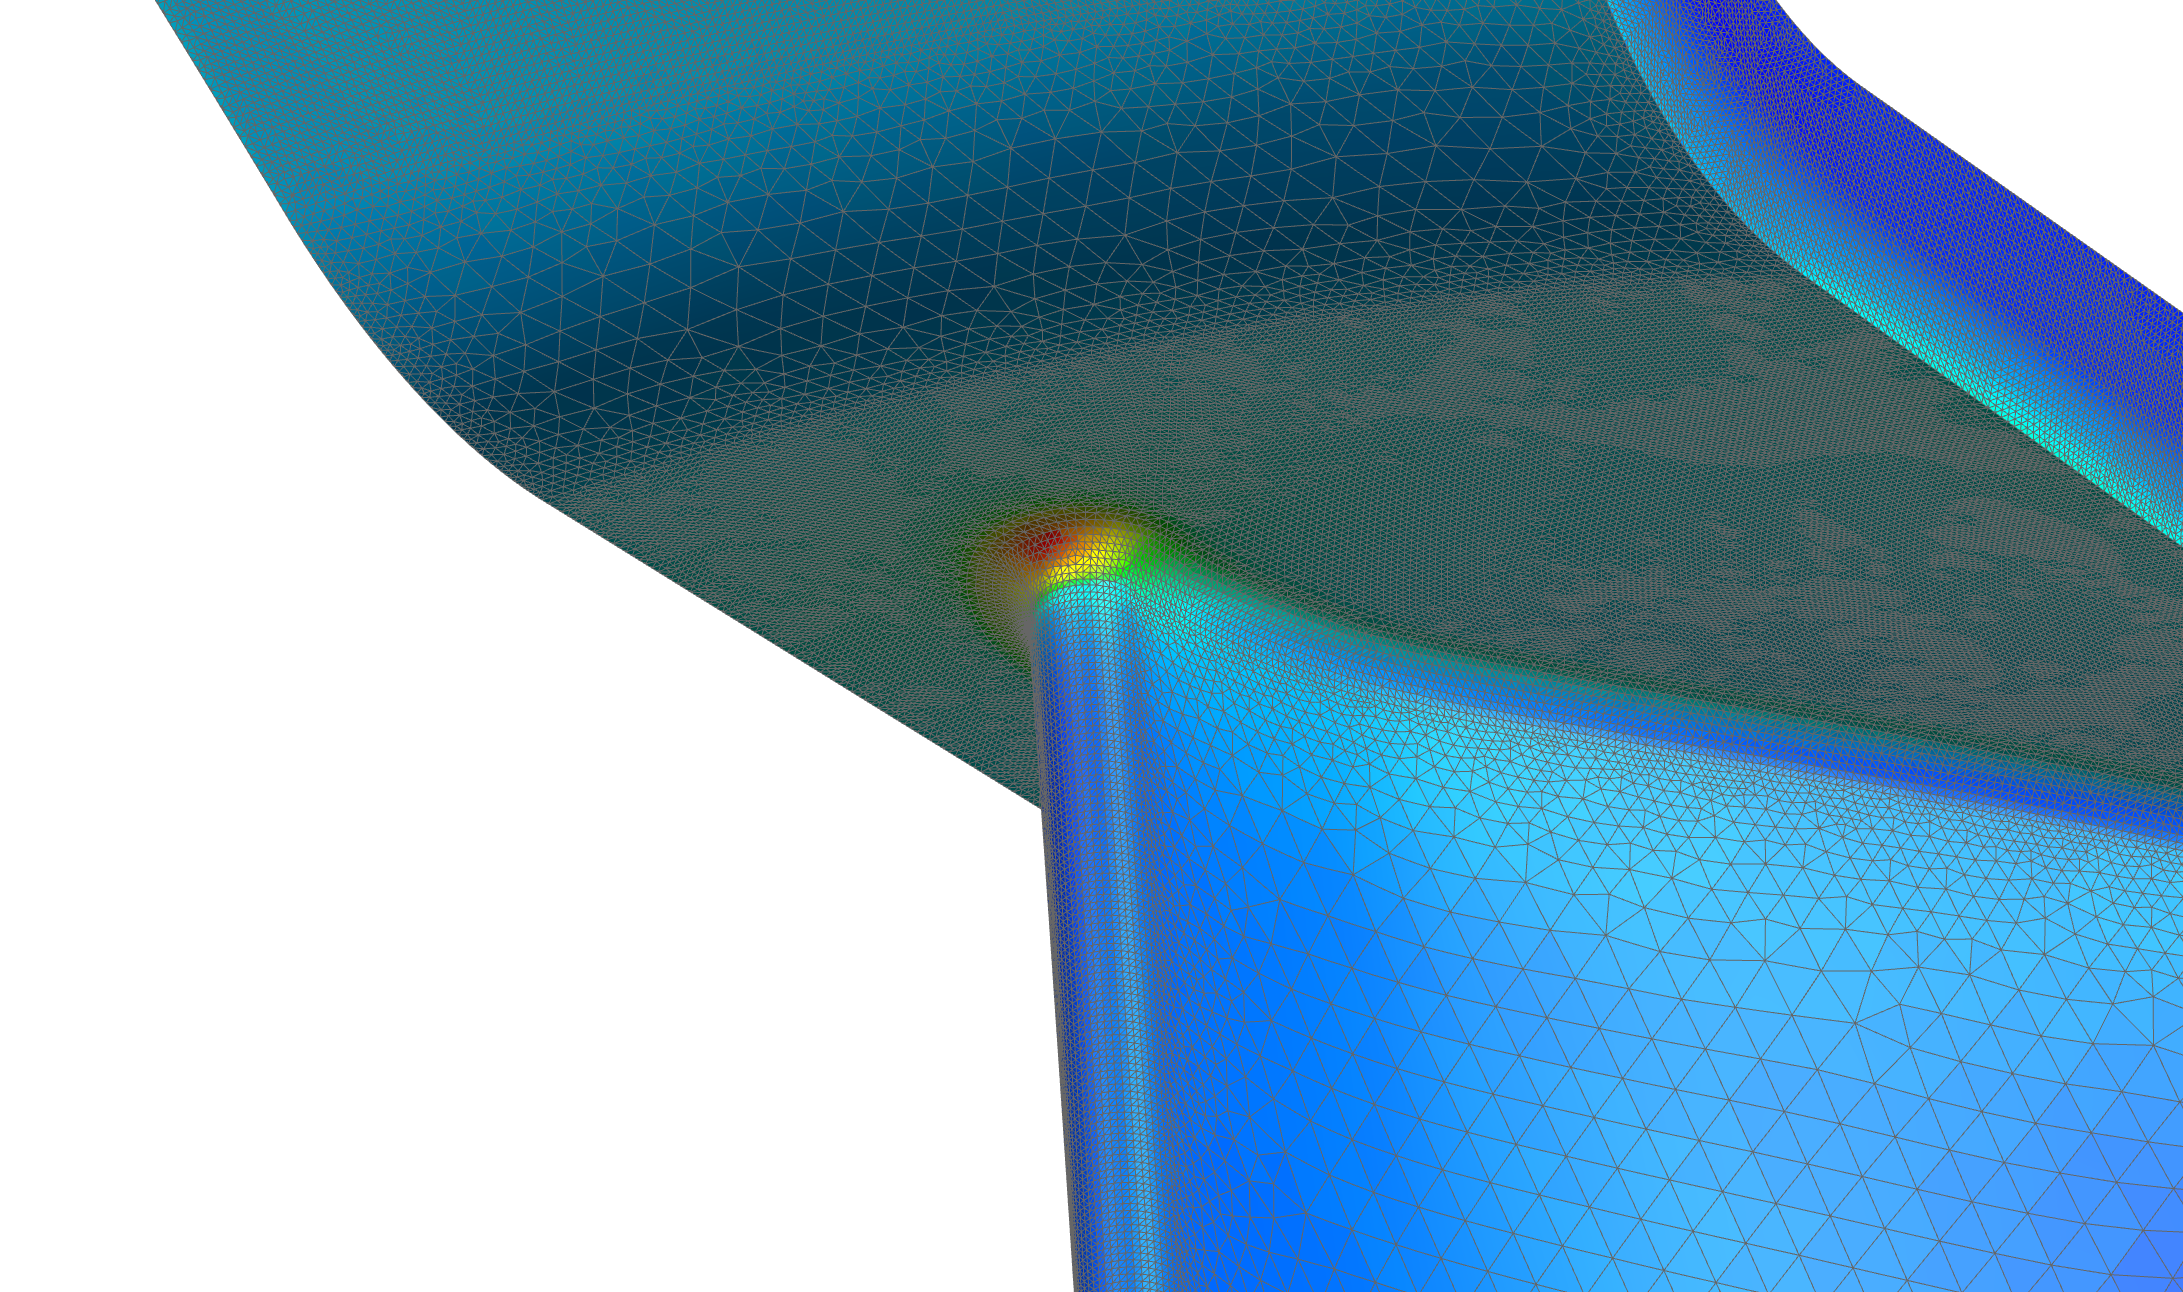
\includegraphics[width=0.8\linewidth]{Figures/stator_shutdown.png}
% 	\caption{Maximum stress during shut-down condition}
%    \label{stator1}
% \end{figure}

\newpage
\section{Battery pack design}
\label{Chap:Battery_Pack_Design}

NX enwat

%\begin{figure} [H]
% 	\centering
% 	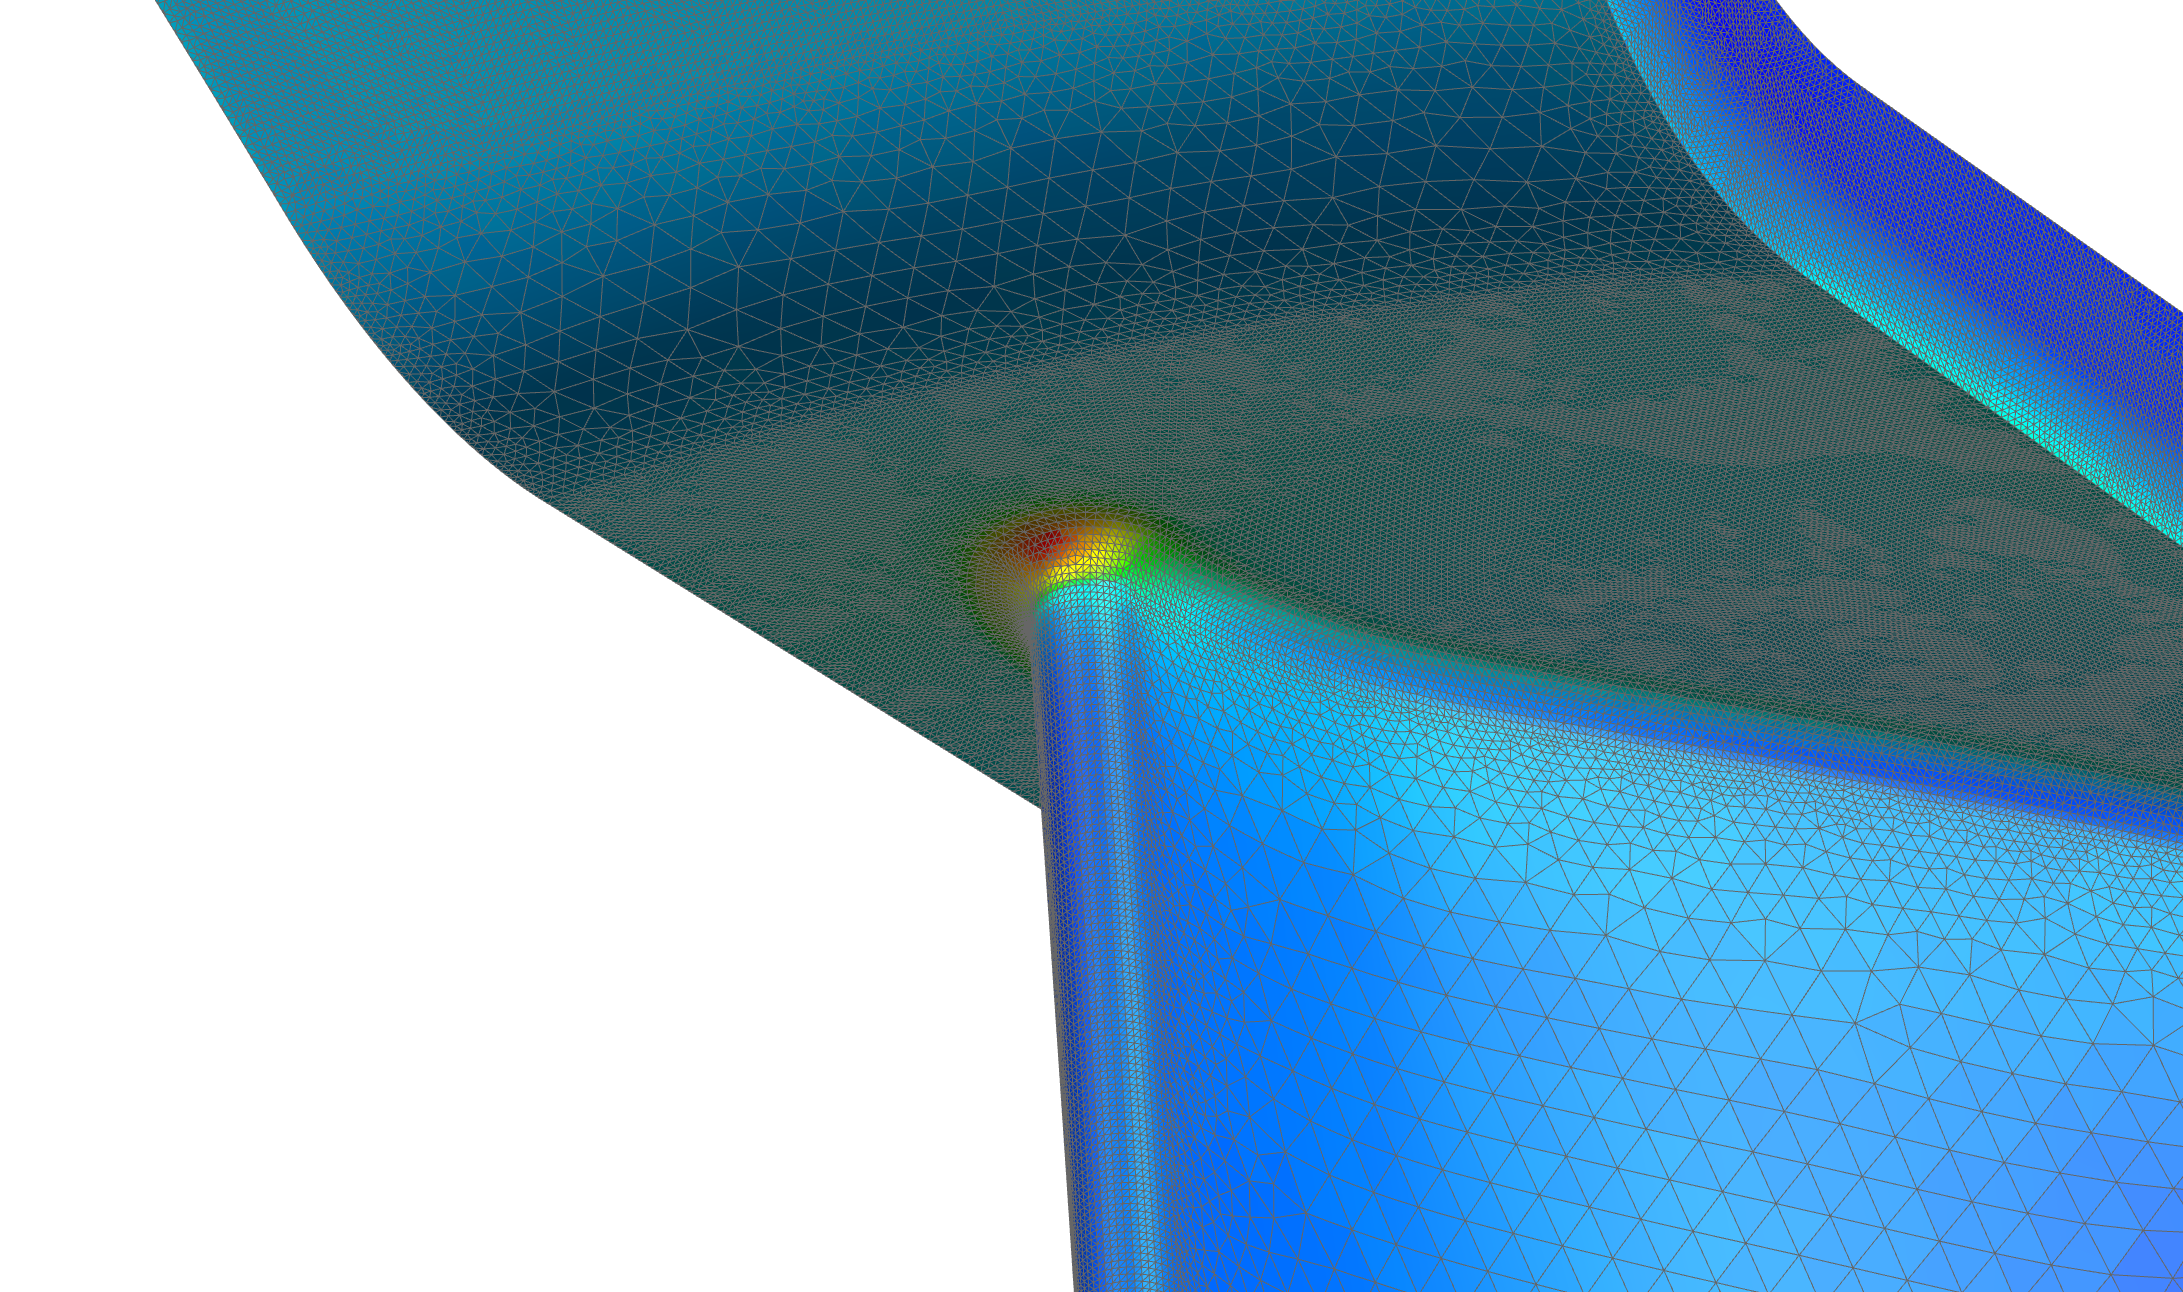
\includegraphics[width=0.8\linewidth]{Figures/stator_shutdown.png}
% 	\caption{Maximum stress during shut-down condition}
%    \label{stator1}
% \end{figure}

\newpage
\input{Sections/Conclusion_Recommendation.tex}
\addcontentsline{toc}{section}{\numberline{}References}
\textit{Later info compleet maken en APA style}

\bibliography{Literature.bib}
\bibliographystyle{unsrt}


\newpage
\newpage
\appendix
\begin{appendices}
\section{Appendix A}
\label{AppendixA}
\subsection{Sample point/lines used in Comsol}

Data is gathered at specific locations in the battery models.
For the 6S1P, the middle point is blabla
\begin{figure} [H]
	\centering
	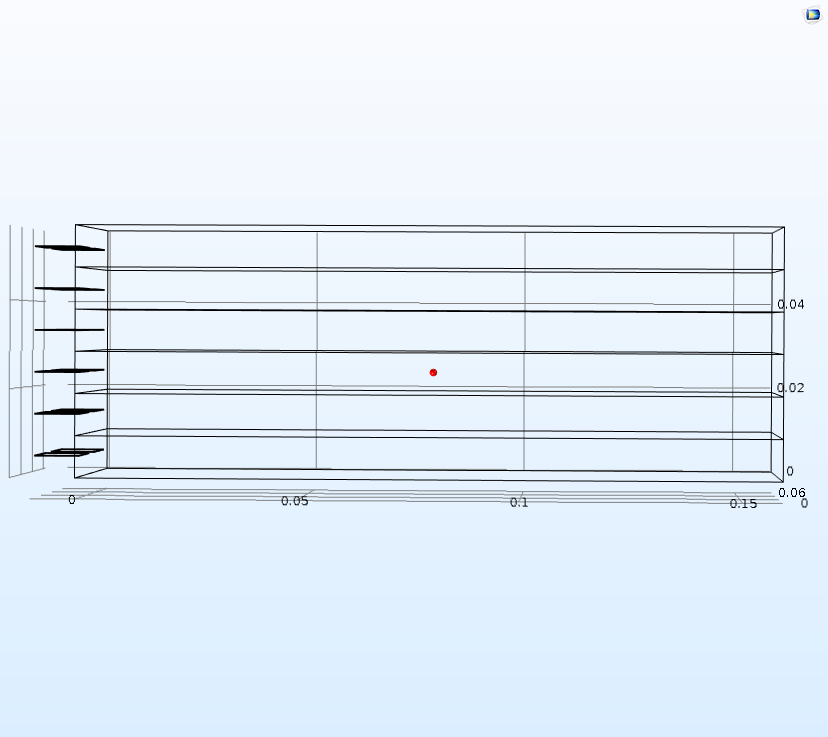
\includegraphics[width=0.5\linewidth]{Figures/6_Point_in_3D.png}
	\caption{Point of measurement in 6S1P simulation.}
   \label{Fig:6_1}
\end{figure}
\begin{figure} [H]
	\centering
	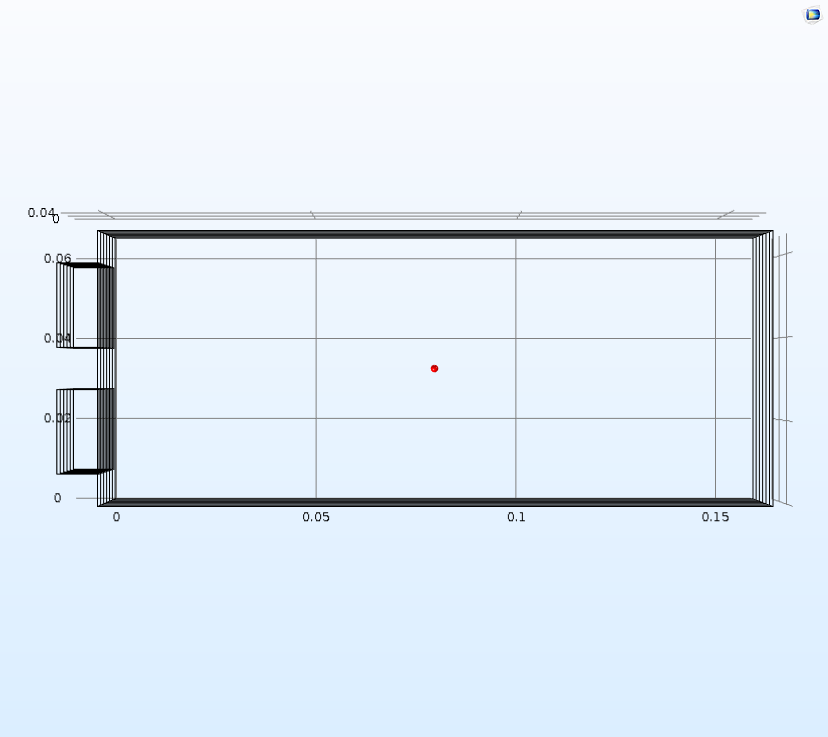
\includegraphics[width=0.5\linewidth]{Figures/6_Point_in_3D_2.png}
	\caption{Point of measurement in 6S1P simulation.}
   \label{Fig:6_2}
\end{figure}

\begin{figure} [H]
	\centering
	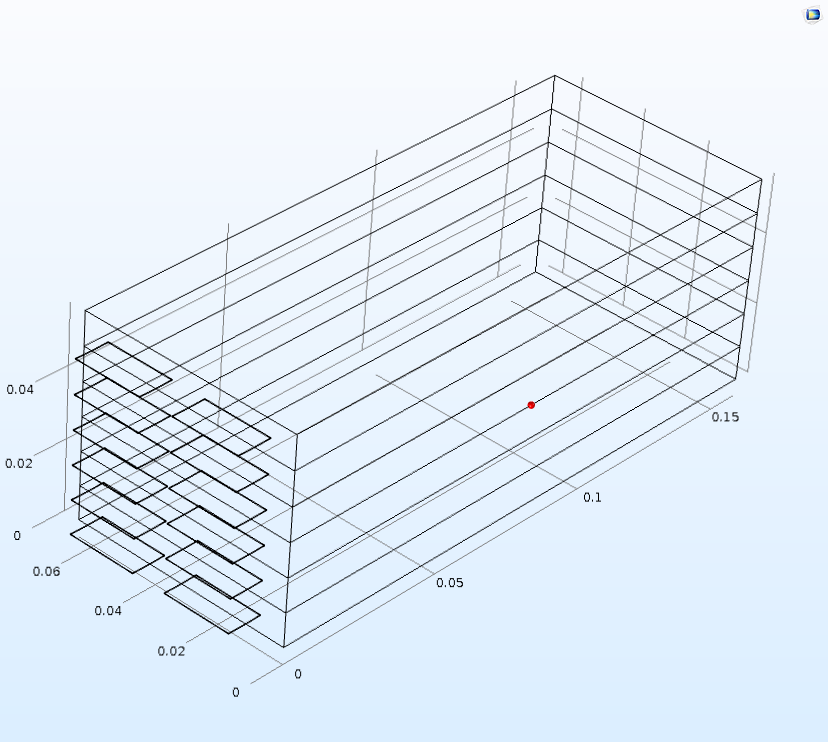
\includegraphics[width=0.5\linewidth]{Figures/6_Point_in_3D_3.png}
	\caption{Point of measurement in 6S1P simulation.}
   \label{Fig:6_3}
\end{figure}

\begin{figure} [H]
	\centering
	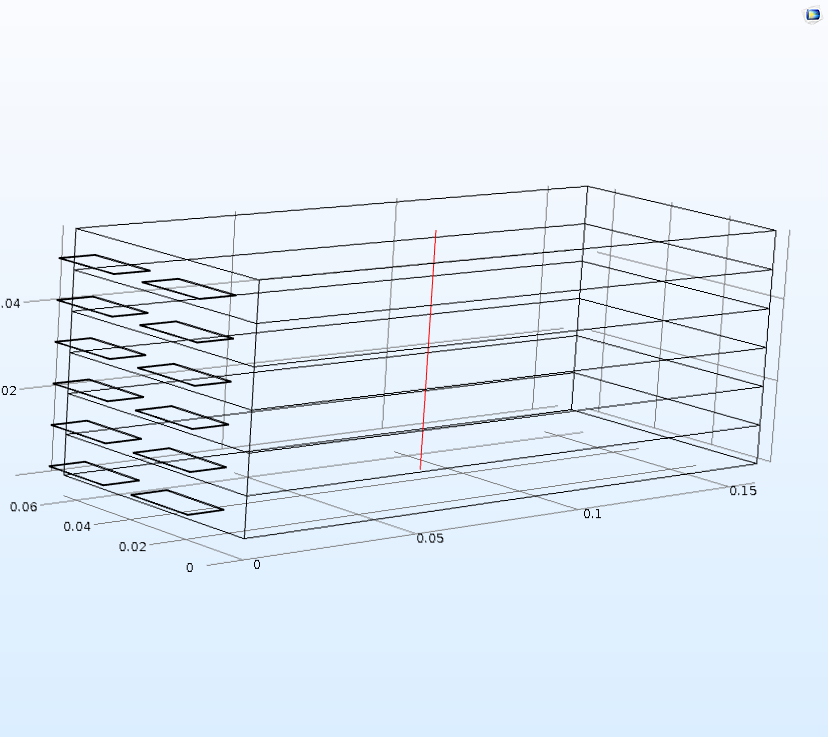
\includegraphics[width=0.5\linewidth]{Figures/LineOutPlane.png}
	\caption{Point of measurement in 6S1P simulation.}
   \label{Fig:6_4}
\end{figure}

\begin{figure} [H]
	\centering
	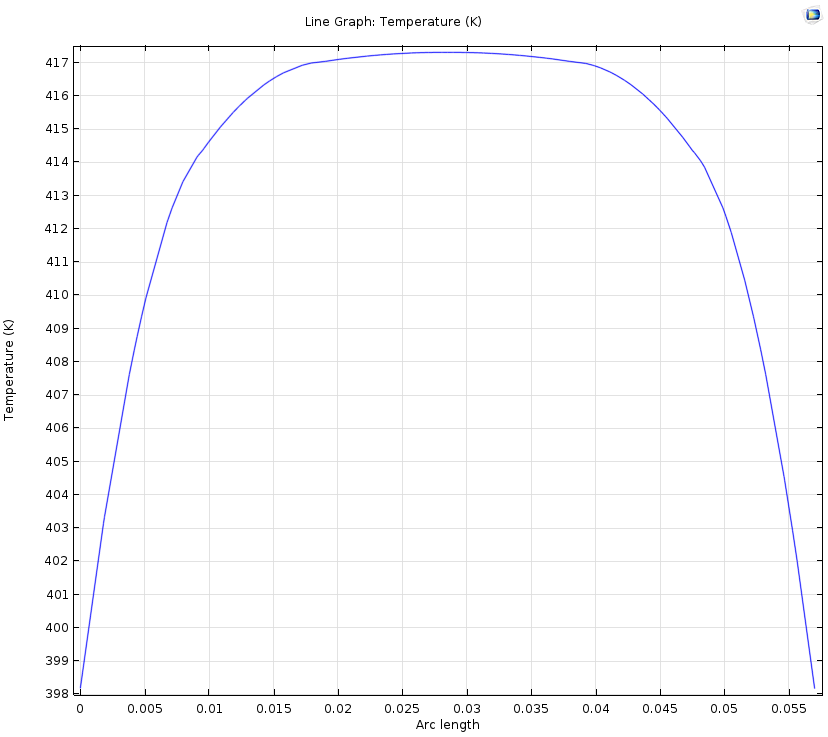
\includegraphics[width=0.5\linewidth]{Figures/300s_10h_180A_2mOhm_OutOfPlaneLast_NoPouch.png}
	\caption{Point of measurement in 6S1P simulation.}
   \label{Fig:6_5}
\end{figure}



\newpage

\end{appendices}

\end{document}
